%
% main.tex
%
% Copyright (C) 2021 by SpaceLab.
%
% OBDH 2.0 Documentation
%
% This work is licensed under the Creative Commons Attribution-ShareAlike 4.0
% International License. To view a copy of this license,
% visit http://creativecommons.org/licenses/by-sa/4.0/.
%

%
% \brief Main file.
%
% \author Gabriel Mariano Marcelino <gabriel.mm8@gmail.com>
%
% \institution Universidade Federal de Santa Catarina (UFSC)
%
% \version 0.6.0
%
% \date 2019/07/18
%

\documentclass[a4paper,12pt]{book}

\usepackage{spacelab_book}

\title{OBDH 2.0 Documentation}
\author{SpaceLab}
\date{\today}

% File metadata
\hypersetup
{
    pdfauthor   = {SpaceLab},
    pdfsubject  = {\thetitle},
    pdftitle    = {\thetitle},
    pdfkeywords = {Nanosatellites, CubeSats, OBDH}
}

\begin{document}

    \pagenumbering{roman}
    \setcounter{page}{1}

    %
% titlepage.tex
%
% Copyright (C) 2022 by SpaceLab.
%
% OBDH 2.0 Module
%
% This work is licensed under the Creative Commons Attribution-ShareAlike 4.0
% International License. To view a copy of this license,
% visit http://creativecommons.org/licenses/by-sa/4.0/.
%

%
% \brief Title page.
%
% \author Gabriel Mariano Marcelino <gabriel.mm8@gmail.com>
% \author Bruno Benedetti <brunobenedetti45@gmail.com>
%
% \version 0.1.0
%
% \date 2022/06/24
%

\begin{frame}
    \titlepage
\end{frame}
    \cleardoublepage
    %
% authorpage.tex
%
% Copyright (C) 2021 by Universidade Federal de Santa Catarina.
%
% OBDH 2.0 Documentation
%
% This work is licensed under the Creative Commons Attribution-ShareAlike 4.0
% International License. To view a copy of this license,
% visit http://creativecommons.org/licenses/by-sa/4.0/.
%

%
% \brief Author page.
%
% \author Gabriel Mariano Marcelino <gabriel.mm8@gmail.com>
%
% \institution Universidade Federal de Santa Catarina (UFSC)
%
% \version 0.9.0
%
% \date 2019/07/18
%

\thispagestyle{empty}

\begin{center}

\textbf{\thetitle}

\textit{November, 2021}

\vspace{1cm}

\textbf{Project Chief:}

Eduardo Augusto Bezerra

\vspace{1cm}

\textbf{Authors:}

Gabriel Mariano Marcelino \\
André Martins Pio de Mattos \\
Yan Castro Azeredo \\

\vspace{1cm}

\textbf{Contributing Authors:}


\vspace{1cm}


\textbf{Revision Control:}

\end{center}

\begin{table}[!ht]
    \begin{center}
        \begin{tabular}{cL{5cm}L{5.5cm}C{2cm}}
            \toprule[1.5pt]
            \textbf{Version} & \textbf{Author(s)} & \textbf{Changes}      & \textbf{Date} \\
            \midrule
            0.1     & Gabriel M. Marcelino        & Document creation     & 10/2019    \\
            0.5     & Gabriel M. Marcelino        & First stable hardware & 08/2020    \\
            0.6     & A. M. P. Mattos, G. M. Marcelino, Y. A. Azeredo & First hardware integration & 04/2021  \\
            0.7     & A. M. P. Mattos, G. M. Marcelino, Y. A. Azeredo & General firmware and hardware improvements & 06/2021      \\
            0.8     & Gabriel M. Marcelino        & Adding the FRAM memory & 10/2021    \\
            0.9     & Gabriel M. Marcelino        & TBC                   & TBC        \\
                    &                             &                       &            \\
            \bottomrule[1.5pt]
        \end{tabular}
    \end{center}
\end{table}

\vfill

\begin{figure}[!h]
	\begin{center}
		\includegraphics[width=0.25\textwidth]{figures/by-sa.eps}
	\end{center}
\end{figure}

\textcopyright\  2021 by Universidade Federal de Santa Catarina. \thetitle. This work is licensed under the Creative Commons Attribution-ShareAlike 4.0 International License. To view a copy of this license, visit \href{http://creativecommons.org/licenses/by-sa/4.0/}{http://creativecommons.org/licenses/by-sa/4.0/}.

    \cleardoublepage

    \listoffigures
    \addcontentsline{toc}{chapter}{List of Figures}

    \listoftables
    \addcontentsline{toc}{chapter}{List of Tables}

    \printnomenclature
    \addcontentsline{toc}{chapter}{Nomenclature}

    \tableofcontents
    \cleardoublepage
    
    \pagenumbering{arabic}
    \setcounter{page}{1}

    %
% introduction.tex
%
% Copyright (C) 2020 by Universidade Federal de Santa Catarina.
%
% OBDH 2.0 Documentation
%
% This work is licensed under the Creative Commons Attribution-ShareAlike 4.0
% International License. To view a copy of this license,
% visit http://creativecommons.org/licenses/by-sa/4.0/.
%

%
% \brief Introduction chapter.
%
% \author Gabriel Mariano Marcelino <gabriel.mm8@gmail.com>
% \author André Martins Pio de Mattos <andrempmattos@gmail.com>
%
% \institution Universidade Federal de Santa Catarina (UFSC)
%
% \version 0.10.0
%
% \date 2019/07/18
%

\chapter{Introduction} \label{ch:introduction}

The OBDH 2.0\nomenclature{\textbf{OBDH}}{\textit{On-Board Data Handling.}} is an On-Board Computer (OBC\nomenclature{\textbf{OBC}}{\textit{On-Board Computer.}}) module designed for nanosatellites. It is one of the service modules developed for the GOLDS-UFSC CubeSat Mission \cite{floripasat2}. The module is responsible for synchronizing actions and the data flow between other modules (i.e., power module, communication module, payloads) and the Earth segment. It packs the generated data into data frames and transmits it back to Earth through a communication module or stores it on non-volatile memory for later retrieval. Commands sent from the Earth segment to the CubeSat are received by radio transceivers located in the communication module and redirected to the OBDH 2.0, which takes the appropriate action or forward the commands to the target module.

The module is a direct upgrade from the OBDH of FloripaSat-1 \cite{obdh-fsat}, which grants a flight heritage rating. The improvements focus on providing a cleaner and more generic implementation compared to the previous version, along with more reliability in software and hardware implementations and adaptations for the new mission requirements. The whole project, including source and documentation files, is available freely on a GitHub repository \cite{obdh2-repo} under the GPLv3 license.


\begin{figure}[!ht]
    \begin{center}
        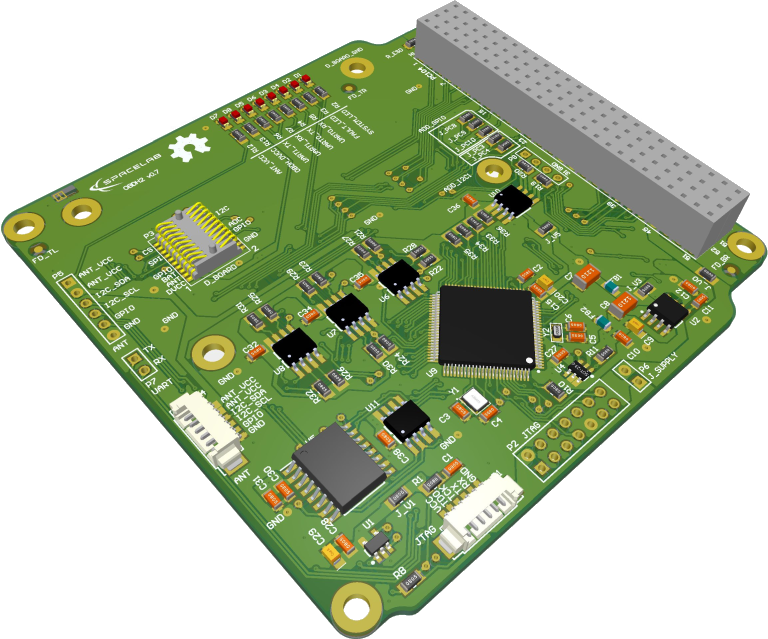
\includegraphics[width=0.65\textwidth]{figures/obdh2-pcb-3d.png}
        \caption{3D view of the OBDH 2.0 PCB\nomenclature{\textbf{PCB}}{\textit{Printed Circuit Board.}}.}
        \label{fig:pcb-3d}
    \end{center}
\end{figure}

    %
% system_overview.tex
%
% Copyright (C) 2019 by SpaceLab.
%
% OBDH 2.0 Documentation
%
% This work is licensed under the Creative Commons Attribution-ShareAlike 4.0
% International License. To view a copy of this license,
% visit http://creativecommons.org/licenses/by-sa/4.0/.
%

%
% \brief System Overview chapter.
%
% \author Gabriel Mariano Marcelino <gabriel.mm8@gmail.com>
% \author André Martins Pio de Mattos <andrempmattos@gmail.com>
%
% \institution Universidade Federal de Santa Catarina (UFSC)
%
% \version 0.10.0
%
% \date 23/11/2019
%

\chapter{System Overview} \label{ch:system-overview}

The board has an MSP430 low-power microcontroller that runs the firmware application and several other peripherals for extended operation and physical interfaces (i.e., non-volatile memory, watchdog timer, service modules, payloads interfaces, daughterboard interface, and current monitor). The microcontroller manages the other sub-modules within the board using serial communication buses, synchronizes actions, handles communication with the ground segment, and manages the data flow. The programming language used is C, and the firmware was developed using the Code Composer Studio IDE\nomenclature{\textbf{IDE}}{\textit{Integrated Development Environment.}} (a.k.a. CCS) for compiling, programming and testing. The module has many tasks over distinct protocols and time requirements, such as interfacing peripherals and other MCUs. To improve predictability, a Real-Time Operating System (RTOS\nomenclature{\textbf{RTOS}}{\textit{Real-Time Operating System.}}) is used to ensure that the deadlines are observed, even under a faulty situation in a routine. The RTOS chosen is the FreeRTOS (v10.0.0), since it is designed for embedded systems applications and was already validated in space applications. The firmware architecture follows an abstraction layer scheme to facilitate higher-level implementations and allow more portability across different hardware platforms.

\section{Product tree}

The product tree of the OBDH 2.0 module is available in \autoref{fig:product-tree}.

\begin{figure}[!ht]
    \begin{center}
        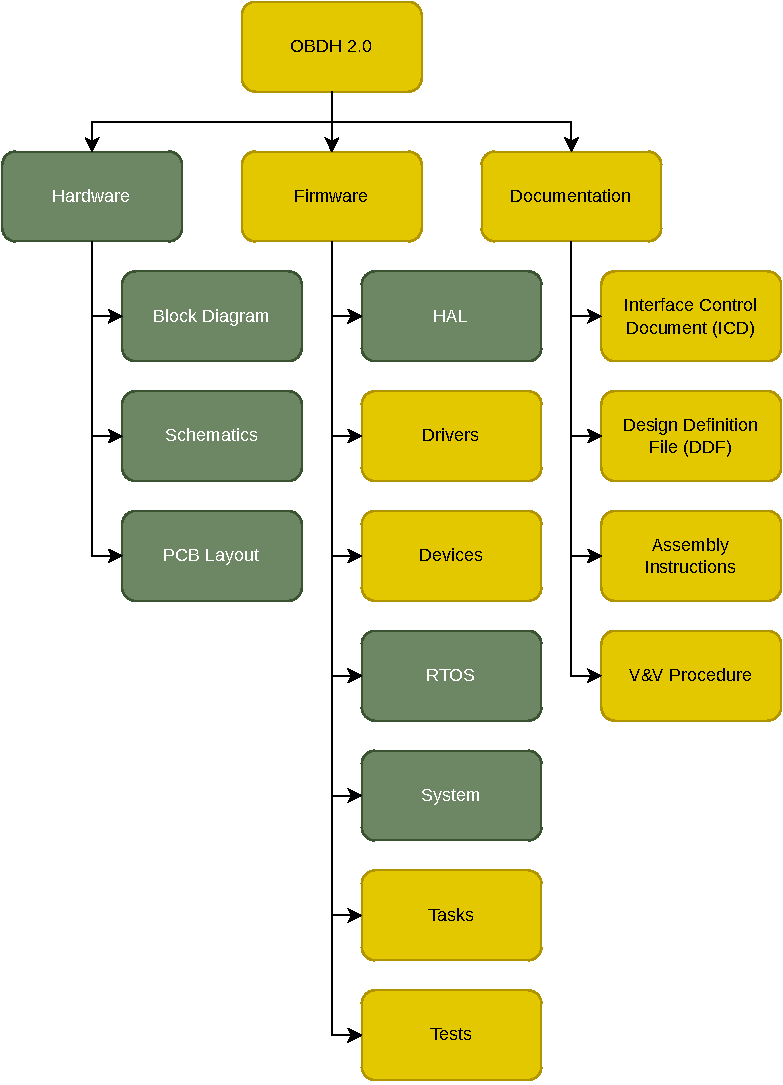
\includegraphics[width=0.8\textwidth]{figures/product-tree.pdf}
        \caption{Product tree of the OBDH 2.0 module.}
        \label{fig:product-tree}
    \end{center}
\end{figure}

\section{Block Diagram}

\autoref{fig:block-diagram} presents a simplified view of the module subsystems and interfaces. The microcontroller has a programming JTAG\nomenclature{\textbf{JTAG}}{\textit{Joint Test Action Group.}}
 and 6 communication buses, divided into 3 different protocols (I2C\nomenclature{\textbf{I2C}}{\textit{Inter-Integrated Circuit.}}, SPI\nomenclature{\textbf{SPI}}{\textit{Serial Peripheral Interface.}}, and UART\nomenclature{\textbf{UART}}{\textit{Universal Asynchronous Receiver/Transmitter.}}), that is shared between all the peripherals and external interfaces. Besides these channels, there are GPIO\nomenclature{\textbf{GPIO}}{\textit{General Purpose Input/Output.}} connections for various functions, from control ports to status pins. There is a non-volatile memory device to store the satellite data frames and critical status indicators. Some buffers and transceivers allow secure and proper communication with external modules. A watchdog timer with a voltage monitor and a current sensor is attached to the system to improve the overall reliability and generate essential housekeeping data. There is a generic daughterboard interface for extending the module capabilities with an auxiliary application board. Also, a UART debug interface is directly connected to the microcontroller. More details and descriptions about these components and interfaces are provided in \autoref{ch:hardware}.

\begin{figure}[!ht]
    \begin{center}
        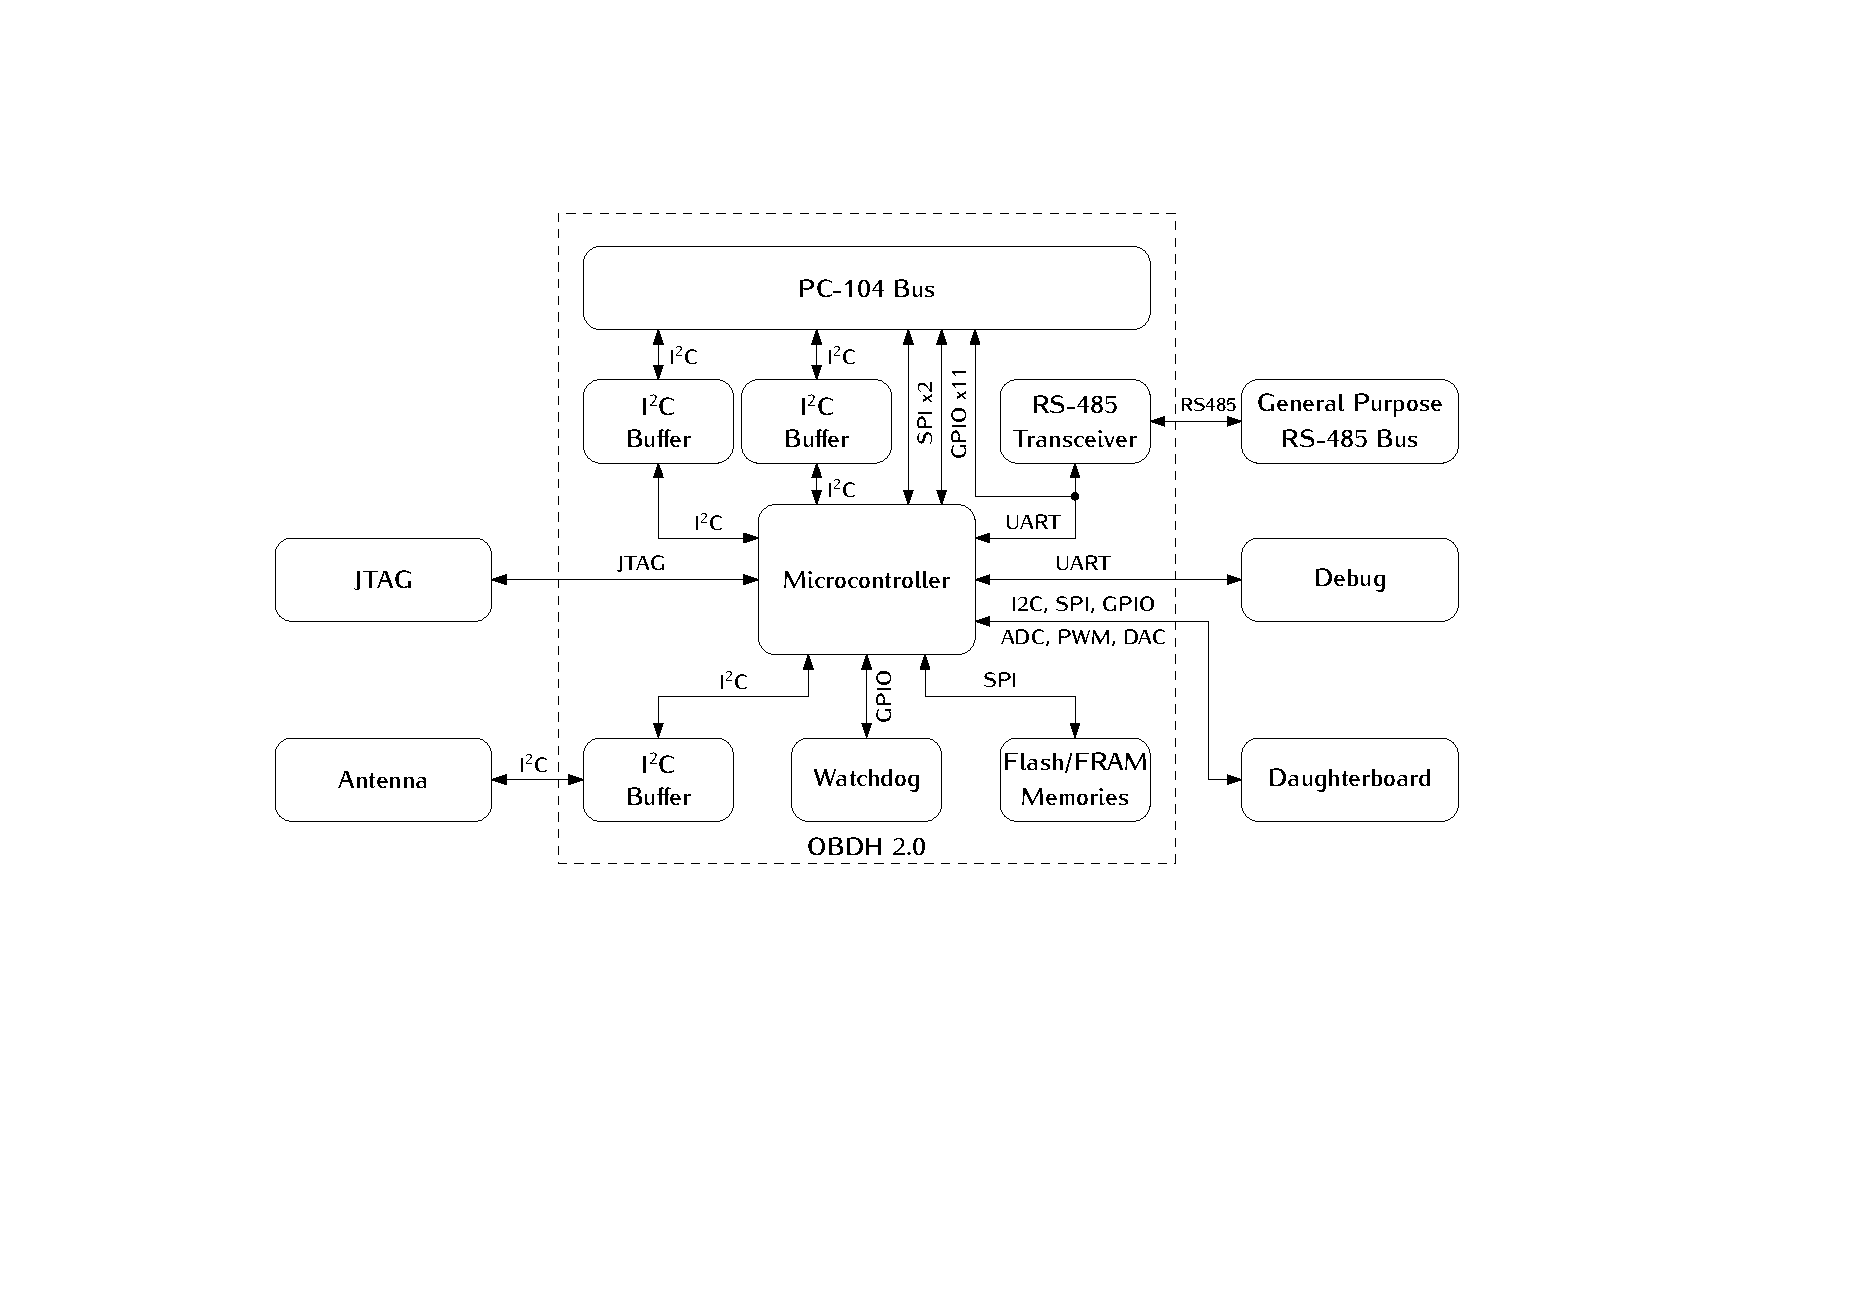
\includegraphics[width=\textwidth]{figures/block_diagram.pdf}
        \caption{OBDH 2.0 Block diagram.}
        \label{fig:block-diagram}
    \end{center}
\end{figure}

\section{System Layers}

As mentioned, the system is divided into abstraction layers to favor high-level firmware implementations. The \autoref{fig:system-layers} shows this scheme, composed of third-party drivers at the lowest layer above the hardware, the operating system as the base building block of the module, the devices handling implementation, and the application tasks in the highest layer. More details are provided in  \autoref{ch:firmware}.

\begin{figure}[!ht]
    \begin{center}
        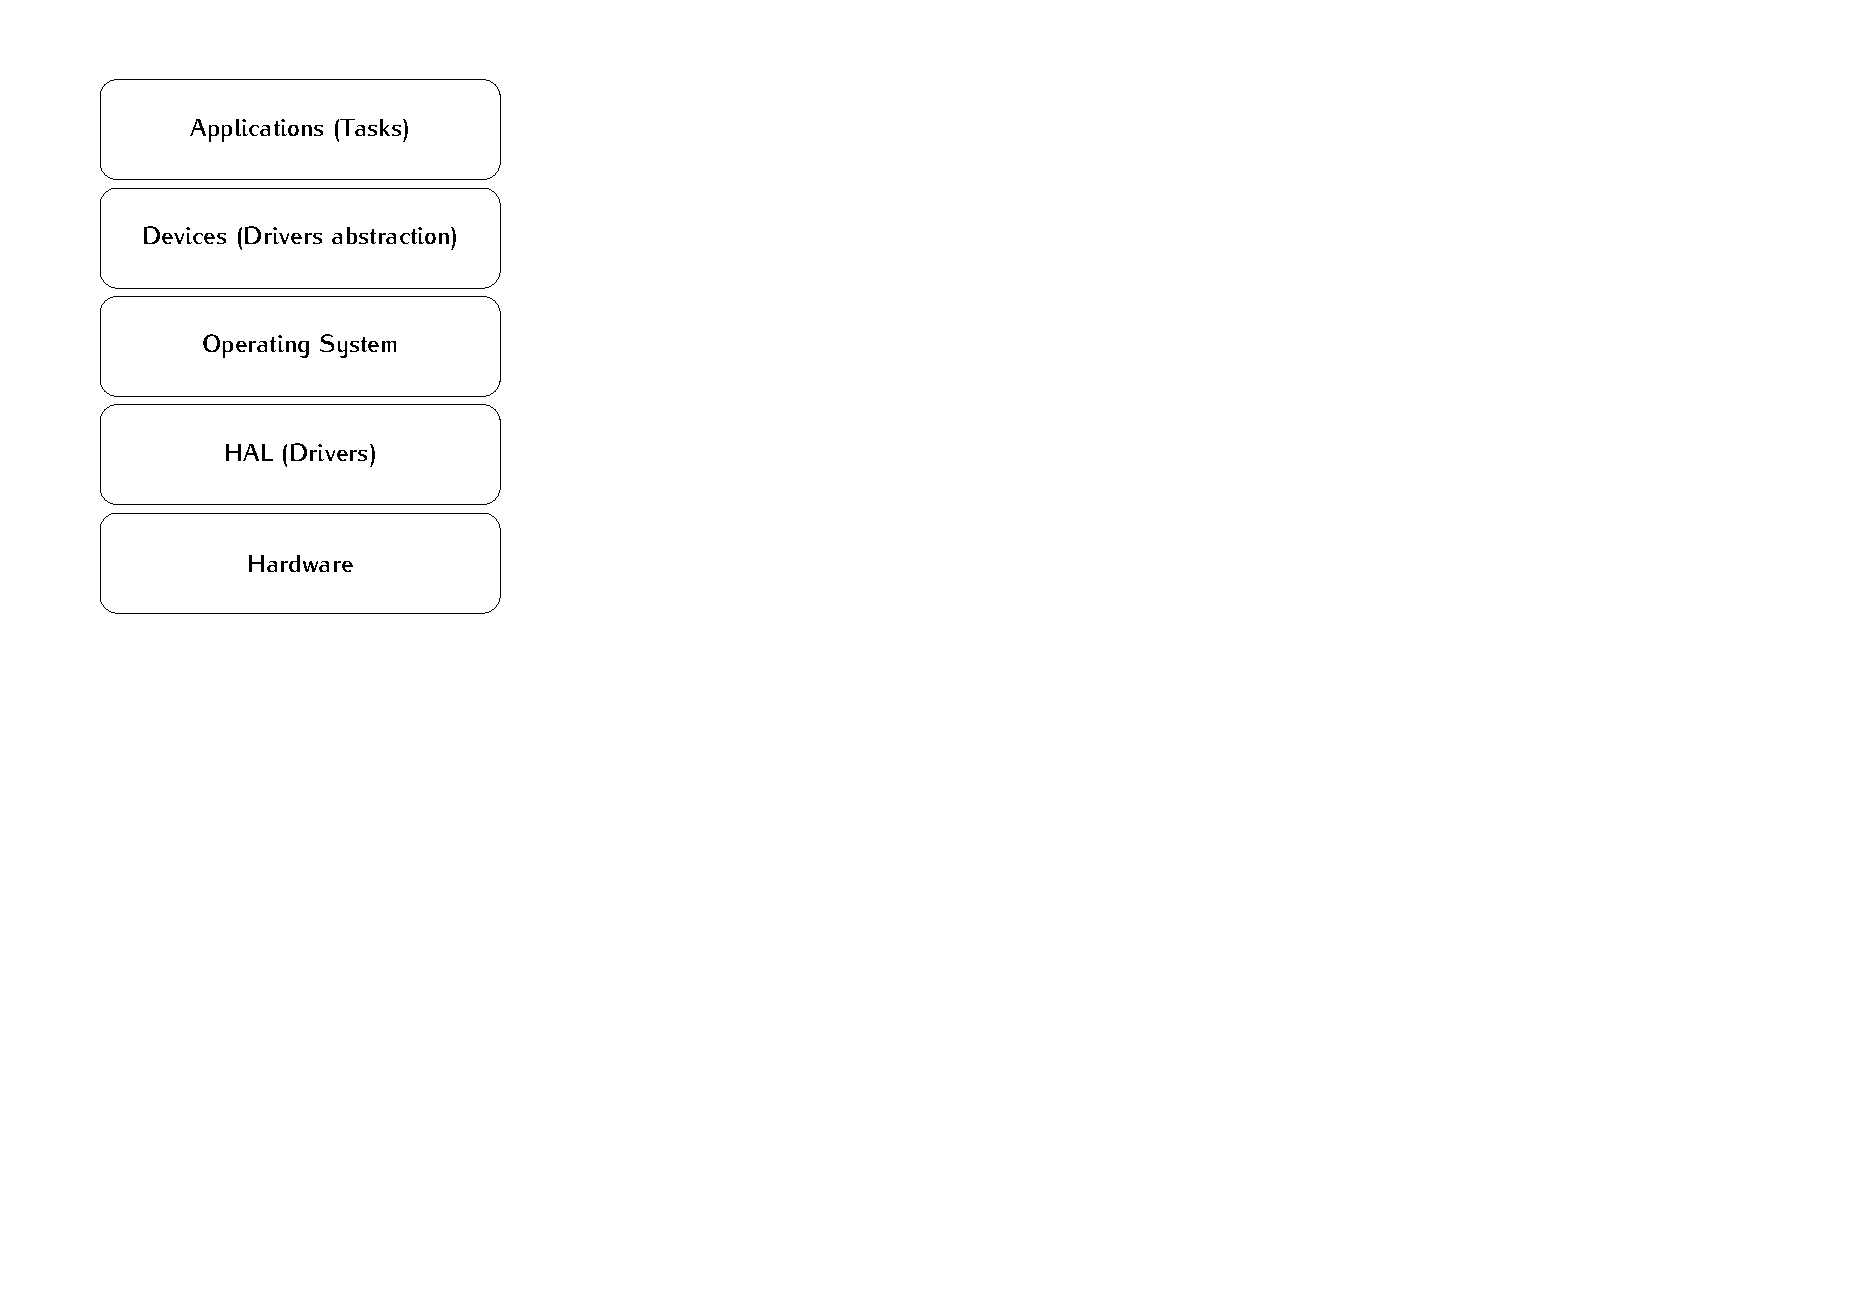
\includegraphics[width=0.4\textwidth]{figures/system_layers.pdf}
        \caption{System layers.}
        \label{fig:system-layers}
    \end{center}
\end{figure}

\section{Operation}

The system operates through the sequential execution of routines (tasks in the context of the operating system) that are scheduled and multiplexed over time. Each routine has a priority and a periodicity, determining the subsequent execution, the set of functionalities currently running, and the memory usage management. Besides this deterministic scheduling system, the routines have communication channels with each other through the usage of queues, which provides a robust synchronization scheme. In \autoref{ch:firmware} the system operation and the internal nuances are described in detail. Then, this section uses a top-view user perspective to describe the module operation.

\subsection{Execution Flow}
% Add here a diagram showing a simple flowchart or use cases to represent how the OBDH works.  
The OBDH 2.0 execution flowchart can be seen on \autoref{fig:flowchart_OBDH}.

\begin{figure}[!ht]
    \begin{center}
        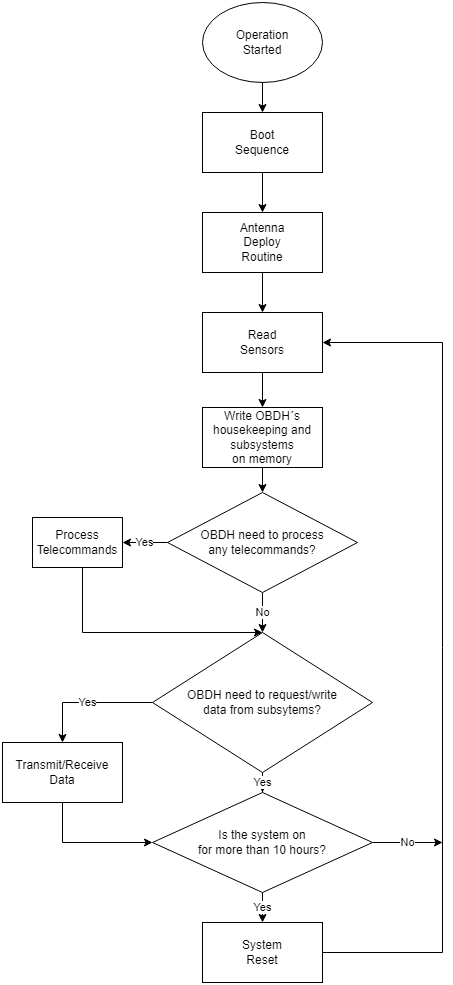
\includegraphics[width=0.6\textwidth]{figures/flowchart_OBDH.drawio.png}
        \caption{OBDH 2.0 operation flowchart}
        \label{fig:flowchart_OBDH}
    \end{center}
\end{figure}

The boot sequence can be seen better on \autoref{fig:flowchart_obdh_boot_sequence}.

\begin{figure}[!ht]
    \begin{center}
        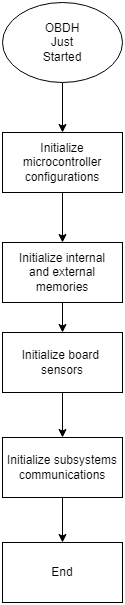
\includegraphics[width=0.2\textwidth]{figures/flowchart_obdh_boot_sequence.drawio.png}
        \caption{OBDH's 2.0 boot sequence.}
        \label{fig:flowchart_obdh_boot_sequence}
    \end{center}
\end{figure}

The antenna deploy routine is exemplified with the flowchart on \autoref{fig:flowchart_antenna_deploy_routine}.

\begin{figure}[!ht]
    \begin{center}
        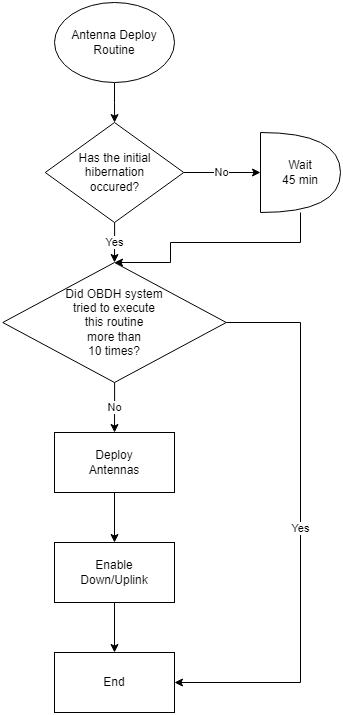
\includegraphics[width=0.45\textwidth]{figures/flowchart_antenna_deploy_routine.png}
        \caption{Antenna deploy routine}
        \label{fig:flowchart_antenna_deploy_routine}
    \end{center}
\end{figure}

The Telecommand's processing flowchart can be seen on \autoref{fig:tc-flowchart}.

\begin{figure}[!ht]
    \begin{center}
        \includegraphics[width=0.75\textwidth]{figures/tc-flowchart.pdf}
        \caption{Telecommand's processing flowchart}
        \label{fig:tc-flowchart}
    \end{center}
\end{figure}

The Transmit/Receive sequence can be seen with the flowchart on \autoref{fig:tx/rx_flowchart}.

\begin{figure}[!ht]
    \begin{center}
        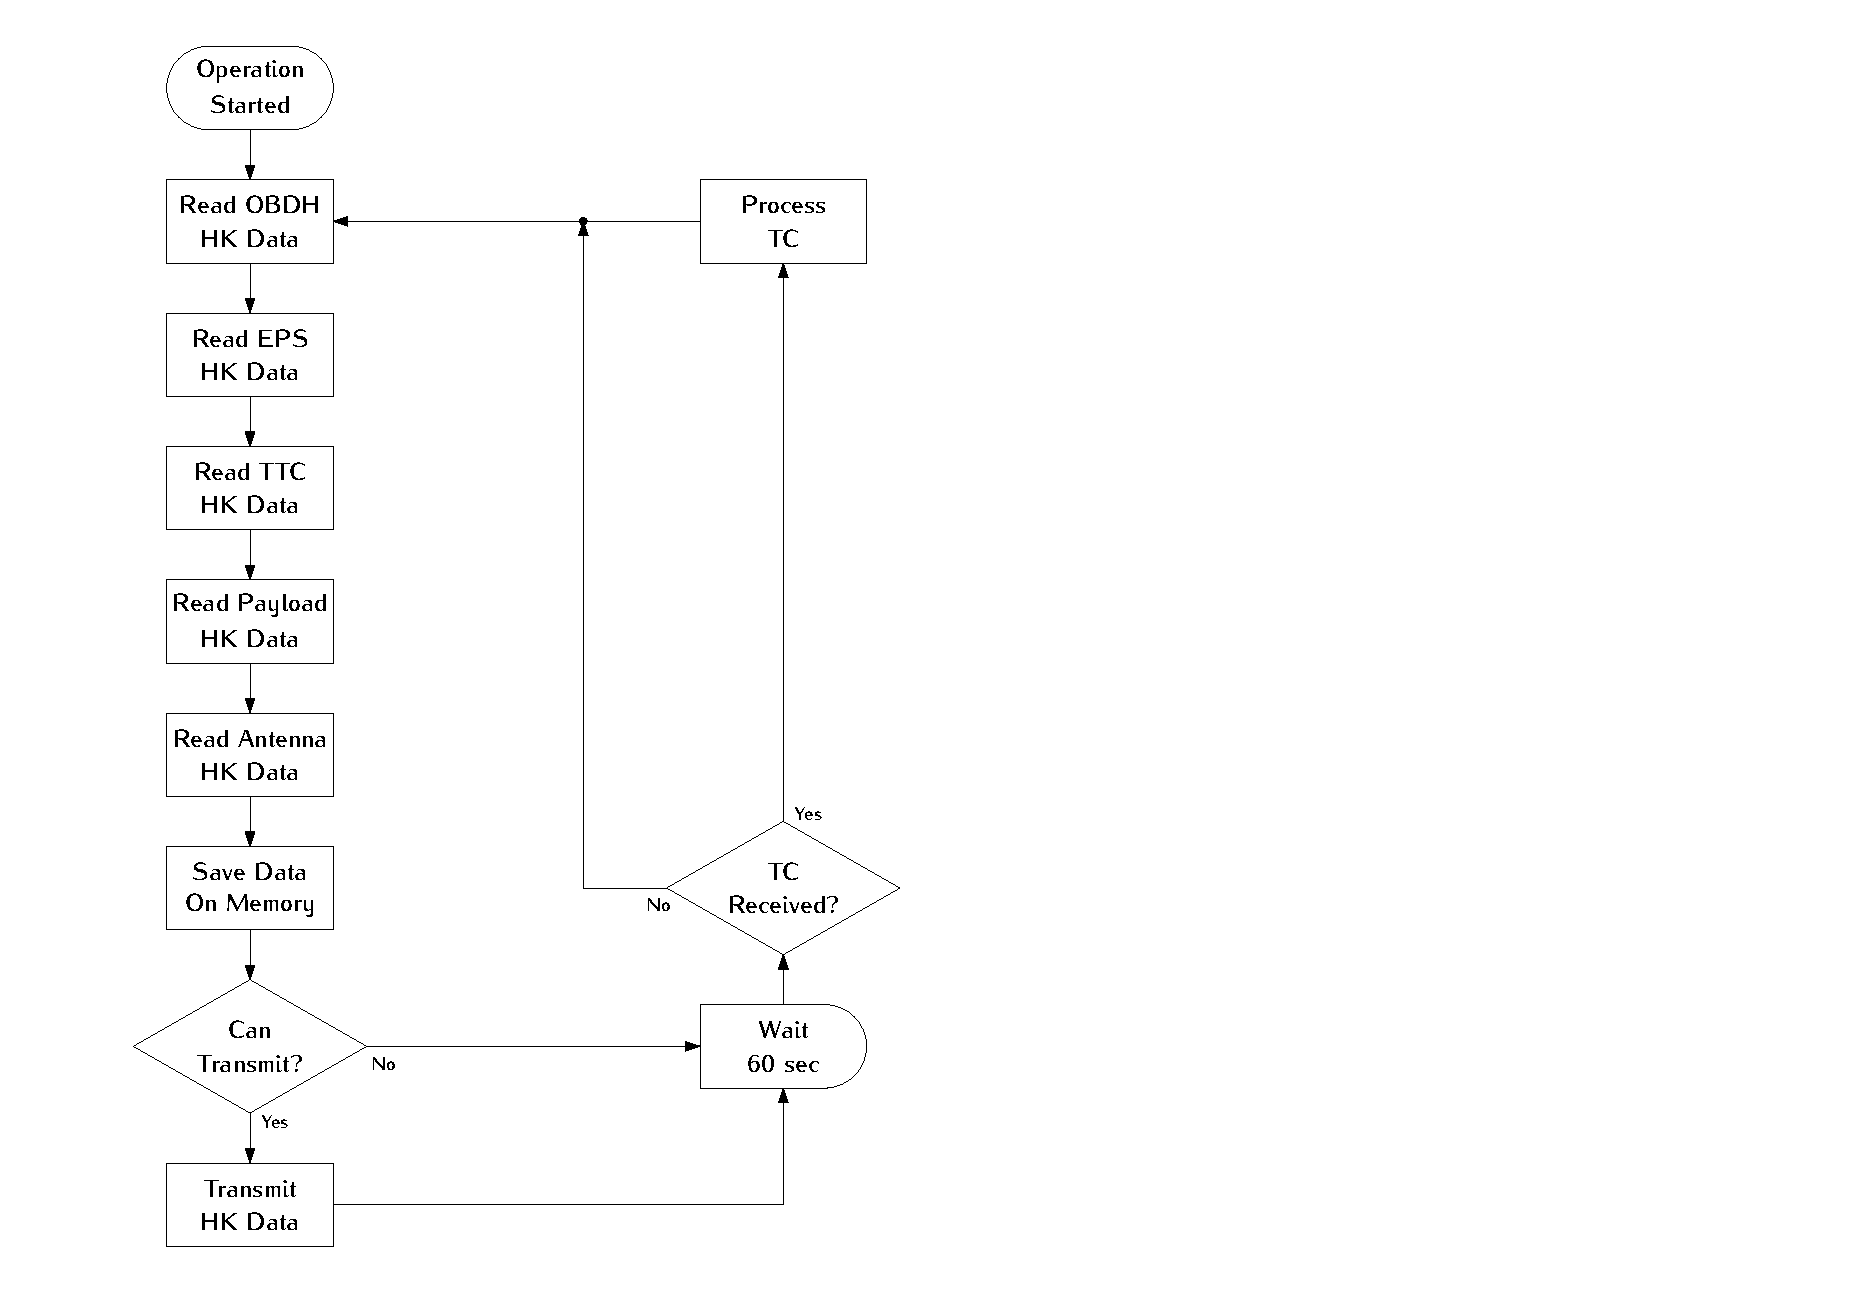
\includegraphics[width=0.55\textwidth]{figures/obdh-flowchart.pdf}
        \caption{Transmit/Receive flowchart}
        \label{fig:tx/rx_flowchart}
    \end{center}
\end{figure}

\subsection{Data Flow}
% Add here a flowchart or diagram showing where and how the data is generated and transferred across different modules and peripherals.

The OBDH 2.0 controls most of the CubeSat's data flow, which can be seen on \autoref{fig:data-path-diagram}.
\begin{figure}[!ht]
    \begin{center}
        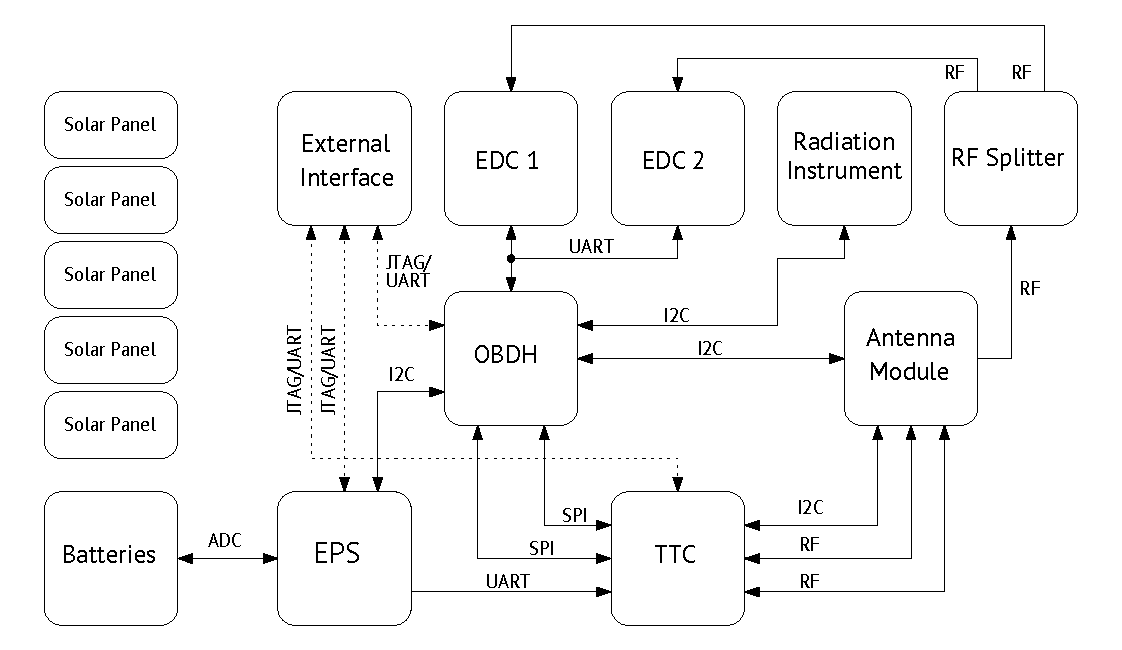
\includegraphics[width=\textwidth]{figures/data_path_diagram.pdf}
        \caption{Data path diagram.}
        \label{fig:data-path-diagram}
    \end{center}
\end{figure}

\subsection{Status LEDs} \label{sec:status-leds}

On the development version of the board, eight LEDs indicate some behaviors of the systems. This set of LEDs can be seen on \autoref{fig:status-leds}.

\begin{figure}[!ht]
    \begin{center}
        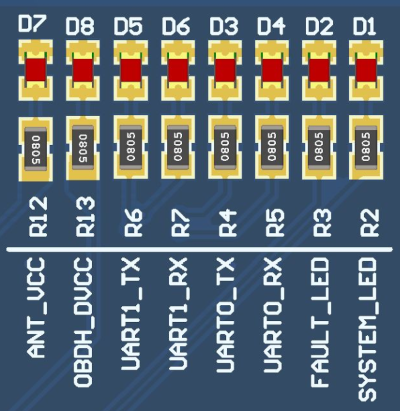
\includegraphics[width=0.3\textwidth]{figures/status_leds.png}
        \caption{Available status LEDs.}
        \label{fig:status-leds}
    \end{center}
\end{figure}

A description of each of these LED\nomenclature{\textbf{LED}}{\textit{Light-Emitting Diode.}}s are available below:

\begin{itemize}
    \item \textbf{D1 - System LED}: Heartbeat of the system. Blinks at a frequency of 1 Hz when the system is running properly.
    \item \textbf{D2 - Fault LED}: Indicates a critical fault in the system.
    \item \textbf{D3 - UART0 TX}: Blinks when data is being transmitted over the UART0 port.
    \item \textbf{D4 - UART0 RX}: Blinks when data is being received over the UART0 port.
    \item \textbf{D5 - UART1 TX}: Blinks when data is being transmitted over that UART1 port.
    \item \textbf{D6 - UART1 RX}: Blinks when data is being received over the UART1 port.
    \item \textbf{D7 - Antenna VCC}: Indicates that the antenna module board is being power sourced.
    \item \textbf{D8 - OBDH VCC}: Indicates that the OBDH board is being power sourced.
\end{itemize}

These LEDs are not mounted in the flight version of the module.

    %
% hardware.tex
%
% Copyright (C) 2020 by Universidade Federal de Santa Catarina.
%
% OBDH 2.0 Documentation
%
% This work is licensed under the Creative Commons Attribution-ShareAlike 4.0
% International License. To view a copy of this license,
% visit http://creativecommons.org/licenses/by-sa/4.0/.
%

%
% \brief Hardware chapter.
%
% \author Gabriel Mariano Marcelino <gabriel.mm8@gmail.com>
% \author André Martins Pio de Mattos <andrempmattos@gmail.com>
%
% \institution Universidade Federal de Santa Catarina (UFSC)
%
% \version 0.8.0
%
% \date 2019/10/20
%

\chapter{Hardware} \label{ch:hardware}

The OBDH 2.0 architecture focus on low-power operation and low-cost production, maintaining performance and proposing different approaches to increase the overall reliability. Therefore, the board was developed using these criteria and the changes from the original design were necessary to improve bottlenecks and achieve the requirements of further space mission. The \autoref{fig:block-diagram} presents the module architecture from the hardware perspective, including the main PCB components and interfaces: microcontroller, buffers, transceivers, memory, watchdog and voltage monitor, and connectors. In the following sections, the hardware design, interfaces, and standards are described in detail. The Figures \ref{fig:pcb-top}, \ref{fig:pcb-bottom} and \ref{fig:pcb-side} present 3D rendered images of the top, bottom and side views of the board, respectively.

\begin{figure}[!ht]
    \begin{center}
        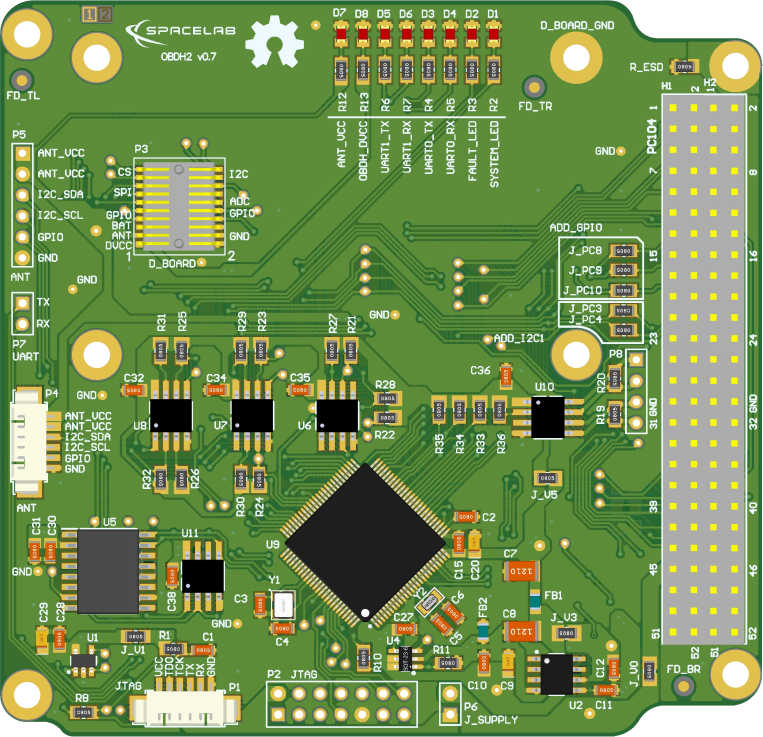
\includegraphics[width=93mm]{figures/obdh2-pcb-top.png}
        \caption{Top side of the PCB.}
        \label{fig:pcb-top}
    \end{center}
\end{figure}

\begin{figure}[!ht]
    \begin{center}
        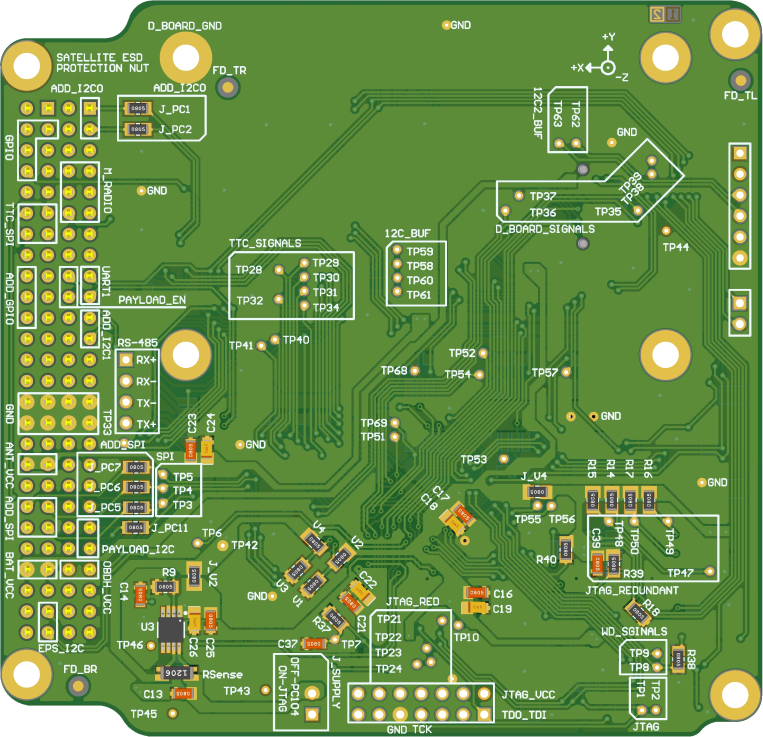
\includegraphics[width=93mm]{figures/obdh2-pcb-bottom.png}
        \caption{Bottom side of the PCB.}
        \label{fig:pcb-bottom}
    \end{center}
\end{figure}

\begin{figure}[!ht]
    \begin{center}
        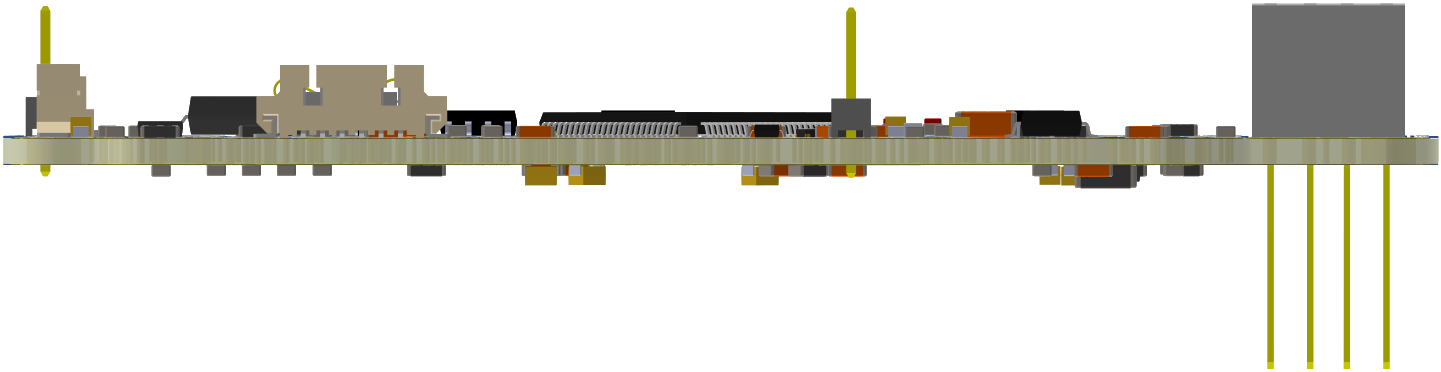
\includegraphics[width=93mm]{figures/obdh2-pcb-side.png}
        \caption{Side view of the PCB.}
        \label{fig:pcb-side}
    \end{center}
\end{figure}


\section{Interfaces}

% Add jtag, daughterboard connector and update the interfaces/payload in the interface diagram

The \autoref{fig:diagram-interfaces} presents the board interfaces, which consists of communication with other modules, debug access points, and internal peripherals. From the perspective of the microcontroller, there are 6 individual and shared communication buses and the JTAG interface, in the following scheme: A0-SPI (shared with Radio, TTC, and external memory chip); A1-UART (shared with redundant payloads); A2-UART (dedicated for debug); B0-I2C (dedicated for the payload); B1-I2C (dedicated for the EPS); B2-I2C (dedicated for the Antenna module). Currently, ``\textit{Payload 1}'' and ``\textit{Payload 2}'' are ``\textit{Payload-X}'' and ``\textit{Payload EDC\nomenclature{\textbf{EDC}}{\textit{Environmental Data Collector.}}}'' respectively.

\begin{figure}[!ht]
    \begin{center}
        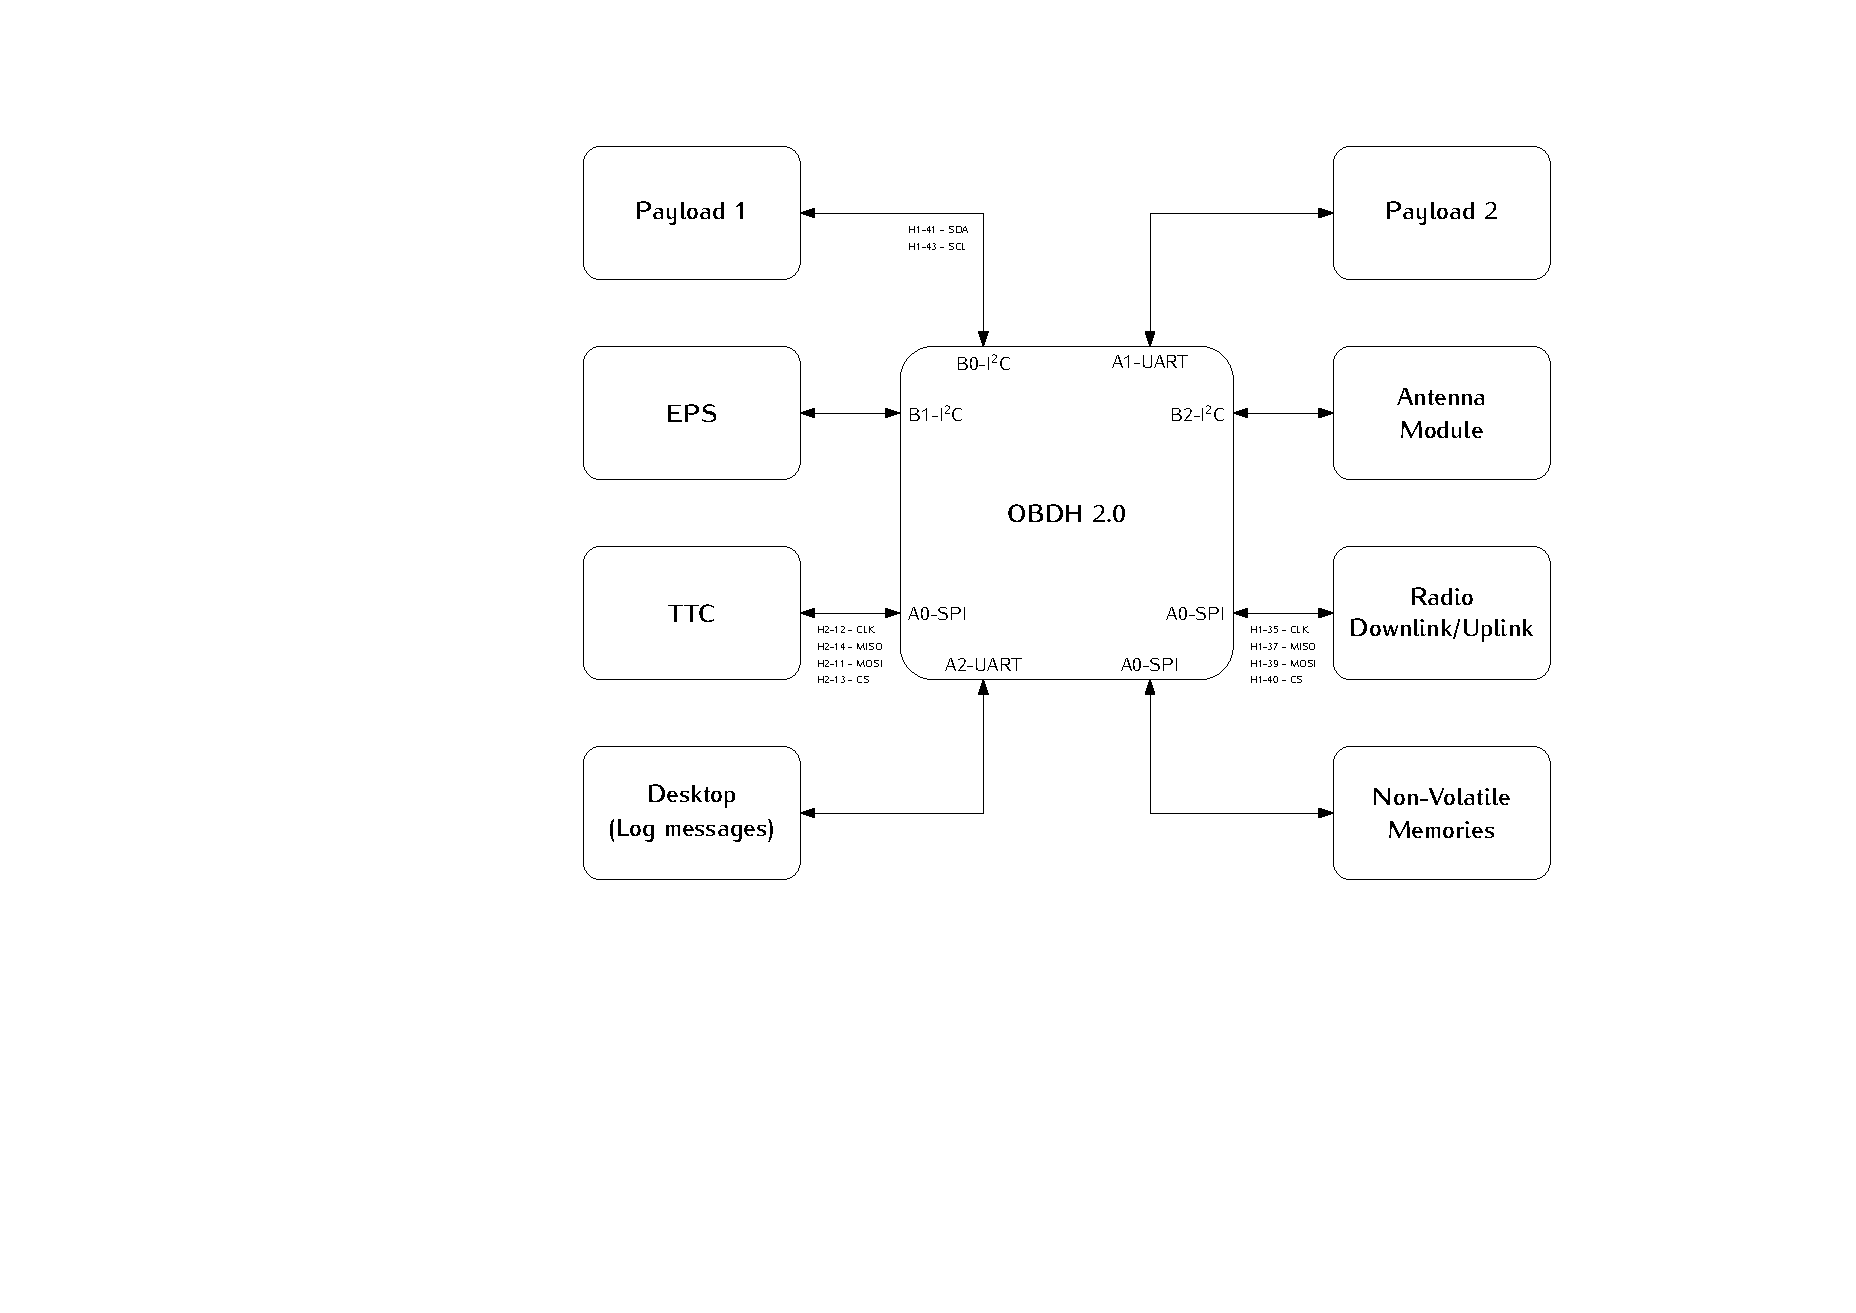
\includegraphics[width=\textwidth]{figures/diagram_interfaces.pdf}
        \caption{Interfaces diagram.}
        \label{fig:diagram-interfaces}
    \end{center}
\end{figure}

\begin{table}[!h]
    \centering
    \begin{tabular}{lrrr}
        \toprule[1.5pt]
        \textbf{Peripheral}     & \textbf{USCI} & \textbf{Protocol} & \textbf{Comm. Protocol} \\
        \midrule
        TTC                     & A0            & SPI               & Register read/write \\
        Radio (downlink/link)   & A0            & SPI               & Radio config./NGHam \\
        NOR Memory              & A0            & SPI               & - \\
        FRAM Memory             & A0            & SPI               & - \\
        Payload port            & A1            & UART              & -\footnotemark \\
        PC (log messages)       & A2            & UART              & ANSI messages \\
        Payload port            & B0            & I$^{2}$C          & -\footnotemark \\
        EPS                     & B1            & I$^{2}$C          & Register read/write \\
        Antenna Module          & B2            & I$^{2}$C          & - \\
        \bottomrule[1.5pt]
    \end{tabular}
    \caption{Boards interfaces.}
    \label{tab:interfaces}
\end{table}

\footnotetext{The communication protocol of the payload ports depends of the used payload.}

\section{External Connectors}

The external interfaces are connected to the microcontroller using different connector types: EPS, TTC, Radio, and Payloads through PC-104; Antenna module with 6H header and 6P picoblade connectors; JTAG through 14H header and 6P picoblade connectors; and debug access using a dedicated 2H header and shared with the JTAG connectors. The following topics describe these interfaces and present the connectors pinout.

\subsection{PC-104} \label{sec:pc104}

% Synchronize nomenclature of the PC-104

The connector referred as PC-104 is a junction of two double row 28H headers (\textit{SSW-126-04-G-D}). These connectors create a solid 104-pin interconnection across the different satellite modules. The \autoref{fig:pc-104-scheme} shows the PC-104 interface from the bottom side of the PCB, which allows visualize the simplified label scheme in the board. Also, the \autoref{tab:pc104-pins} provides the connector pinout\footnote{This pinout is simplified since additional interfaces were omitted. Refer to \textit{option sheet} in chapter \ref{ch:assembly}.} for the pins that are connected to the module. 

\begin{figure}[!ht]
    \begin{center}
        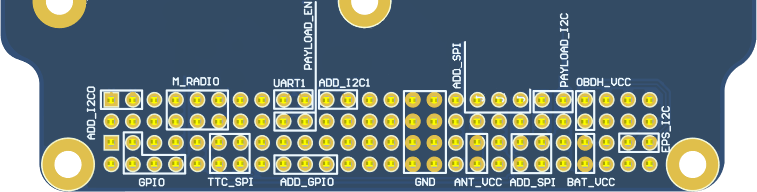
\includegraphics[width=0.75\textwidth]{figures/pc-104-scheme.png}
        \caption{Bottom view of PC-104 and simplified labels}
        \label{fig:pc-104-scheme}
    \end{center}
\end{figure}

\begin{table}[!h]
    \centering
    \begin{tabular}{cllll}
        \toprule[1.5pt]
        \textbf{Pin [A-B]} & \textbf{H1A}     & \textbf{H1B}     & \textbf{H2A}  & \textbf{H2B}  \\
        \midrule
        1-2                & -                & -                & -             & -             \\
        3-4                & -                & -                & GPIO\_4       & GPIO\_5       \\
        5-6                & -                & -                & -             & -             \\
        7-8                & GPIO\_0          & GPIO\_1          & -             & GPIO\_6       \\
        9-10               & GPIO\_2          & -                & -             & -             \\
        11-12              & GPIO\_3          & GPIO\_7          & SPI\_0\_MOSI  & SPI\_0\_CLK   \\
        13-14              & -                & -                & SPI\_0\_CS\_1 & SPI\_0\_MISO  \\
        15-16              & -                & -                & -             & -             \\
        17-18              & UART\_1\_RX      & GPIO\_8          & -             & -             \\
        19-20              & UART\_1\_TX      & GPIO\_9          & -             & -             \\
        21-22              & -                & -                & -             & -             \\
        23-24              & -                & -                & -             & -             \\
        25-26              & -                & -                & -             & -             \\
        27-28              & -                & -                & -             & -             \\
        29-30              & GND              & GND              & GND           & GND           \\
        31-32              & GND              & GND              & GND           & GND           \\
        33-34              & -                & -                & -             & -             \\
        35-36              & SPI\_0\_CLK      & -                & VCC\_3V3\_ANT & VCC\_3V3\_ANT \\
        37-38              & SPI\_0\_MISO     & -                & -             & -             \\
        39-40              & SPI\_0\_MOSI     & SPI\_0\_CS\_0    & -             & -             \\
        41-42              & I2C\_0\_SDA      & -                & -             & -             \\
        43-44              & I2C\_0\_SCL      & -                & -             & -             \\
        45-46              & VCC\_3V3         & VCC\_3V3         & VCC\_BAT      & VCC\_BAT      \\
        47-48              & -                & -                & -             & -             \\
        49-50              & -                & -                & I2C\_1\_SDA   & -             \\
        51-52              & -                & -                & I2C\_1\_SCL   & -             \\
        \bottomrule[1.5pt]
    \end{tabular}
    \caption{PC-104 connector pinout.}
    \label{tab:pc104-pins}
\end{table}

\subsection{Antenna Module}

The communication with the Antenna module is performed through external connectors, which are presented in the \autoref{fig:ant-connectors}. Both connectors have the same connections, but the \ref{fig:ant-debug-connector} (6H header) is used for development and the \ref{fig:ant-main-connector} (6P picoblade) as the connector for the flight model. This interface consists of a dedicated I2C, power supply, and GPIO, which are described in the \autoref{tab:antenna-connector-pins}.

\begin{table}[!h]
    \centering
    \begin{tabular}{cllll}
        \toprule[1.5pt]
        \textbf{Pin} & \textbf{Row} \\
        \midrule
        1            & VCC\_3V3\_ANT  \\
        2            & VCC\_3V3\_ANT  \\
        3            & I2C\_SDA       \\
        4            & I2C\_SCL       \\
        5            & GPIO           \\
        6            & GND            \\
        \bottomrule[1.5pt]
    \end{tabular}
    \caption{Antenna module connectors pinout.}
    \label{tab:antenna-connector-pins}
\end{table}

\begin{figure}[!htb]
    \begin{center}
        \subfigure[Debug interface of the antenna module.\label{fig:ant-debug-connector}]{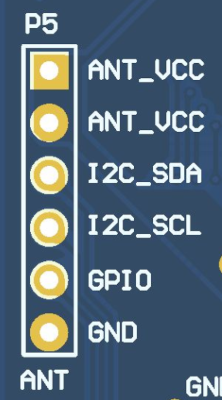
\includegraphics[width=0.135\textwidth]{figures/p5-connector.png}}
        \qquad
        \subfigure[Main interface of the antenna module.\label{fig:ant-main-connector}]{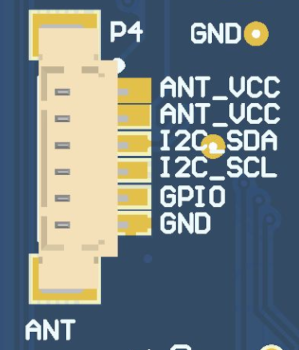
\includegraphics[width=0.205\textwidth]{figures/p4-connector.png}}
        \caption{Antenna module conectors.}
        \label{fig:ant-connectors}
    \end{center}
\end{figure}

\subsection{Programmer and Debug} \label{sec:programer-and-debug}

The interface with the microcontroller programmer is performed through external connectors, which are presented in the \autoref{fig:jtag-connectors}. Both connectors have the same JTAG and UART interfaces, but the 14H header is used during development and the 6P picoblade (provide more compact and reliable attachment) as the connector for the flight model, which are described in the \autoref{tab:jtag-header-connector-pins} and \autoref{tab:jtag-picoblade-connector-pins}, respectively. This interface consists of a dedicated debug UART, a JTAG, and an external power supply. The debug UART connection has another access point in a dedicated 2H header (P7), as shown in \autoref{fig:uart-debug-connector}. Also, to use this external supply, it is necessary to connect both pins of a 2H header jumper (P6).

\begin{figure}[!ht]
    \begin{center}
        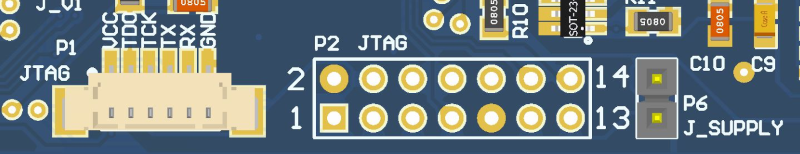
\includegraphics[width=0.7\textwidth]{figures/jtag-connector.png}
        \caption{Programmer (P1 and P2) and jumper (P6) connectors.}
        \label{fig:jtag-connectors}
    \end{center}
\end{figure}

\begin{table}[!h]
    \centering
    \begin{tabular}{cllll}
        \toprule[1.5pt]
        \textbf{Pin [A-B]} & \textbf{Row A} & \textbf{Row B} \\
        \midrule
        1-2                & TDO\_TDI       & VCC\_3V3       \\
        3-4                & -              & -              \\
        5-6                & -              & -              \\
        7-8                & TCK            & -              \\
        9-10               & GND            & -              \\
        11-12              & -              & UART\_TX       \\
        13-14              & -              & UART\_RX       \\
        \bottomrule[1.5pt]
    \end{tabular}
    \caption{Programmer header connector pinout.}
    \label{tab:jtag-header-connector-pins}
\end{table}

\begin{table}[!h]
    \centering
    \begin{tabular}{cllll}
        \toprule[1.5pt]
        \textbf{Pin} & \textbf{Row} \\
        \midrule
        1            & VCC\_3V3       \\
        2            & TDO\_TDI       \\
        3            & TCK            \\
        4            & UART\_TX       \\
        5            & UART\_RX       \\
        6            & GND            \\
        \bottomrule[1.5pt]
    \end{tabular}
    \caption{Programmer picoblade connector pinout.}
    \label{tab:jtag-picoblade-connector-pins}
\end{table}

\begin{figure}[!ht]
    \begin{center}
        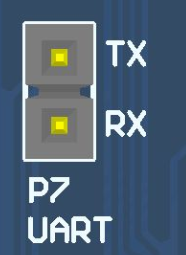
\includegraphics[width=0.15\textwidth]{figures/p7-connector.png}
        \caption{Dedicated UART debug connectors (P7).}
        \label{fig:uart-debug-connector}
    \end{center}
\end{figure}

\subsection{Daughterboard} \label{sec:daughterboard-interface}

The daughterboard interface uses the Samtec FSI-110-D connector \cite{fsi-conn}, which can be seen in the \autoref{fig:samtec-connector}. This connector has metal contacts in format of arcs that are flexible and four polymer guide pins (a pair for top and bottom). When the daughterboard is attached, there is some pressure to this metal contacts that bend and create a meaningful pin connection to the daughterboard copper pads\footnote{These daughterboard pads are similar to the ones used as footprint in the OBDH, despite a slightly bigger size.}. A picture of this connector on the PCB can be seen in \autoref{fig:daughterboard-connector}.

\begin{figure}[!ht]
    \begin{center}
        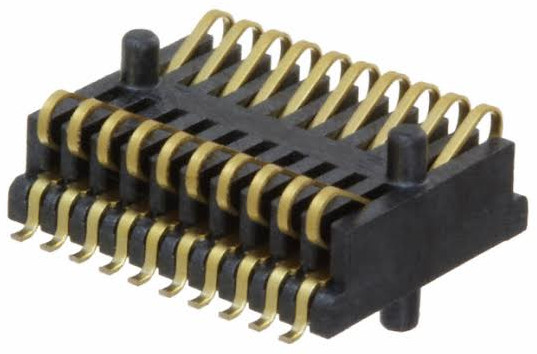
\includegraphics[width=0.4\textwidth]{figures/samtec_fsi-110-03-g-d-ad.jpeg}
        \caption{Samtec FSI-110-03-G-D-AD connector.}
        \label{fig:samtec-connector}
    \end{center}
\end{figure}

\begin{figure}[!ht]
    \begin{center}
        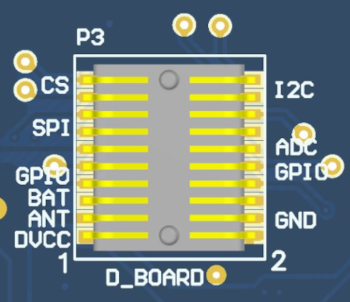
\includegraphics[width=0.3\textwidth]{figures/p3-connector.png}
        \caption{Daughterboard connector (P3).}
        \label{fig:daughterboard-connector}
    \end{center}
\end{figure}

The pinout of the daughterboard interface are available in the \autoref{tab:daugtherboard-connector-pins}. There are different power supply lines (OBDH, Antenna, and battery), communication buses (I2C and SPI), GPIO, and ADC\nomenclature{\textbf{ADC}}{\textit{Analog-to-Digital Converter.}} interfaces available. Besides the GPIO and ADC pins, the other interfaces are shared with other modules and peripherals.

\begin{table}[!h]
    \centering
    \begin{tabular}{cllll}
        \toprule[1.5pt]
        \textbf{Pin [A-B]} & \textbf{Row A} & \textbf{Row B} \\
        \midrule
        1-2                & VCC\_3V3       & GND            \\
        3-4                & VCC\_3V3\_ANT  & GND            \\
        5-6                & VCC\_BAT       & GND            \\
        7-8                & GPIO\_0        & GPIO\_1        \\
        9-10               & GPIO\_2        & GPIO\_3        \\
        11-12              & SPI\_0\_CLK    & ADC\_0         \\
        13-14              & SPI\_0\_MISO   & ADC\_1         \\
        15-16              & SPI\_0\_MOSI   & ADC\_2         \\
        17-18              & SPI\_0\_CS\_0  & I2C\_2\_SDA    \\
        19-20              & SPI\_0\_CS\_1  & I2C\_2\_SCL    \\
        \bottomrule[1.5pt]
    \end{tabular}
    \caption{Daughterboard connector pinout.}
    \label{tab:daugtherboard-connector-pins}
\end{table}

\subsubsection{Guidelines}

The recommended shape and size of the daughterboard can be seen in the \autoref{fig:daughterboard-size}. Besides that, there are mandatory and suggested elements placement: four M3 holes for mechanical attachment, required; contact connector pads (in light gray on the bottom layer), required; two debug headers in the left and bottom sides, suggested; and a general purpose flight model picoblade, suggested.

\begin{figure}[!ht]
    \begin{center}
        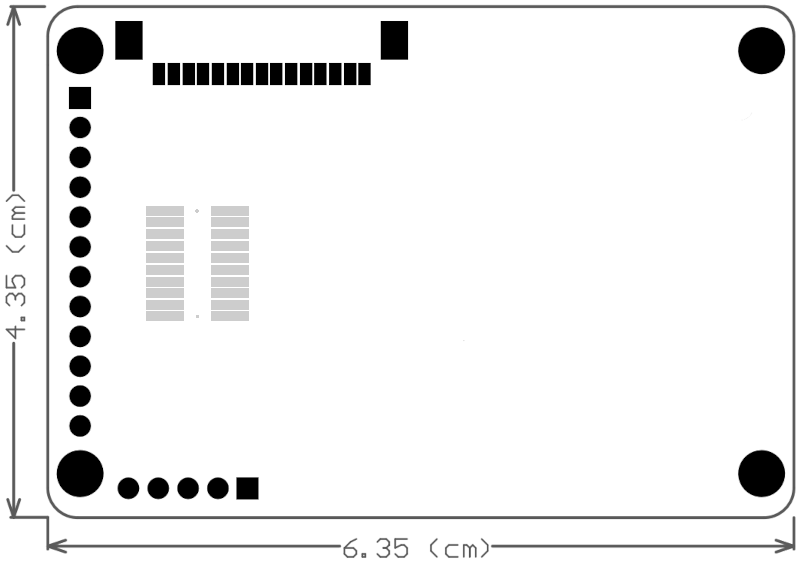
\includegraphics[width=0.52\textwidth]{figures/daughterboard-size.png}
        \caption{Recommended shape and size of the daughterboard.}
        \label{fig:daughterboard-size}
    \end{center}
\end{figure}

\begin{figure}[!ht]
    \begin{center}
        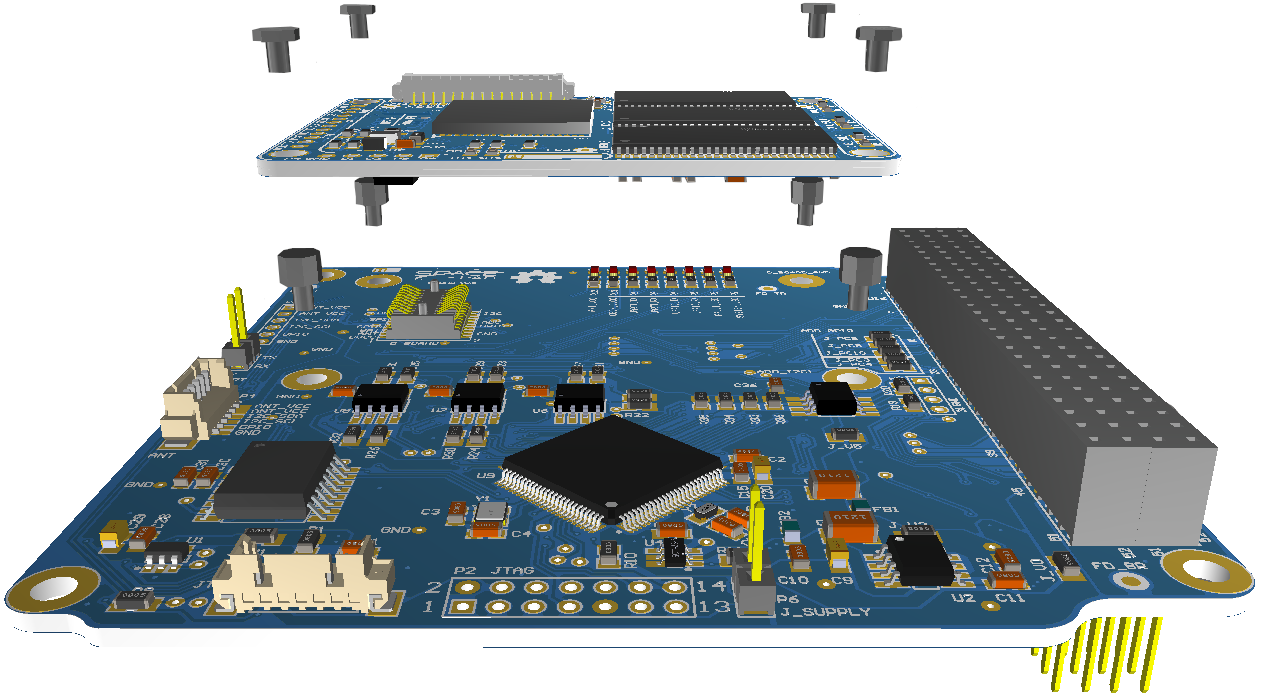
\includegraphics[width=0.6\textwidth]{figures/daughterboard-integration.png}
        \caption{Illustrative daughterboard integration.}
        \label{fig:daughterboard-integration}
    \end{center}
\end{figure}

\section{Microcontroller}

The OBDH 2.0 uses a low-power and low-cost microcontroller family from Texas Instruments, the MSP430F6659 \cite{msp430f6659}. This device provide sufficient performance for low and medium complexity software and algorithms, allowing the module to execute the required tasks. The \autoref{tab:msp430-summary} presents a summary of the main available features and \autoref{fig:msp430-diagram} shows the internal subsystems, descriptions, and peripherals. The microcontroller interfaces, configurations, and auxiliary components are described in the following topics.

\begin{table}[!h]
    \centering
    \begin{tabular}{cllllllll}
        \toprule[1.5pt]
        \textbf{Flash} & \textbf{SRAM} & \textbf{Timers} & \textbf{USCI} & \textbf{ADC} & \textbf{DAC} & \textbf{GPIO} \\
        \midrule
        512KB  & 64KB  & 2  & 6 (SPI / I2C / UART)  & 12  & 2  & 74           \\
        \bottomrule[1.5pt]
    \end{tabular}
    \caption{Microcontroller features summary.}
    \label{tab:msp430-summary}
\end{table}

\begin{figure}[!ht]
    \begin{center}
        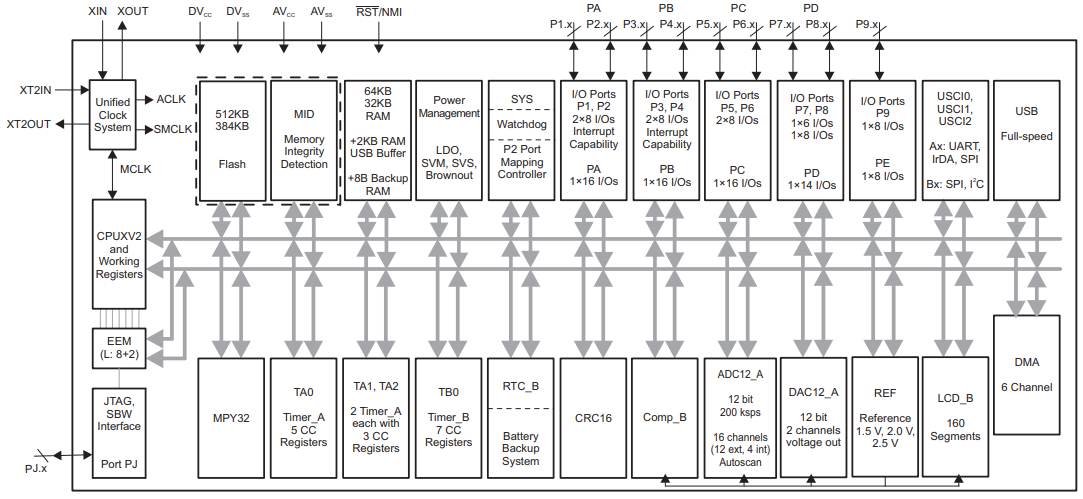
\includegraphics[width=\textwidth]{figures/msp430-diagram.png}
        \caption{Microcontroller internal diagram.}
        \label{fig:msp430-diagram}
    \end{center}
\end{figure}

\subsection{Interfaces Configuration}

The microcontroller has 6 Universal Serial Communication Interfaces (USCI\nomenclature{\textbf{USCI}}{\textit{Universal Serial Communication Interfaces.}}) that can be configured to operate with different protocols and parameters. These interfaces are connected to different modules and peripherals, as presented in the \autoref{fig:diagram-interfaces}. The \autoref{tab:usci-config} describes each interface configurations.

\begin{table}[!h]
    \centering
    \begin{tabular}{lrrrrl}
        \toprule[1.5pt]
        \textbf{Interface} & \textbf{Protocol (Index)} & \textbf{Mode} & \textbf{Word Length} & \textbf{Data Rate} & \textbf{Configuration} \\
        \midrule
        USCI\_A0           & SPI                       & Master        & 8 bits               & 1 Mbps             & Phase: High \\
                           &                           &               &                      &                    & Polarity: Low \\
        USCI\_A1           & UART1                     & -             & 8 bits               & 115200 bps         & Stop bits: 1 \\
                           &                           &               &                      &                    & Parity: None \\
        USCI\_A2           & UART0                     & -             & 8 bits               & 115200 bps         & Stop bits: 1 \\
                           &                           &               &                      &                    & Parity: None \\
        USCI\_B0           & I2C0                      & Master        & 8 bits               & 100 kbps           & Adr. len: 7 bits \\
        USCI\_B1           & I2C1                      & Master        & 8 bits               & 100 kbps           & Adr. len: 7 bits \\
        USCI\_B2           & I2C2                      & Master        & 8 bits               & 100 kbps           & Adr. len: 7 bits \\
        \bottomrule[1.5pt]
    \end{tabular}
    \caption{USCI configuration.}
    \label{tab:usci-config}
\end{table}

\subsection{Clocks Configuration}

Besides the internal clock sources, the microcontroller has two dedicated clock inputs for external crystals: the main clock and the auxiliary clock inputs. There are a $32\ MHz$ crystal and a $32.769\ kHz$ connected to these inputs, respectively. The first source is used for generating the Master Clock (MCLK) and the Subsystem Master Clock (SMCLK), which are used by the CPU and the internal peripheral modules. The second source is used for generating the Auxiliary Clock (ACLK) that handles the low-power modes and might be used for peripherals.

\subsection{Pinout}

An illustration of the microcontroller pinout positions can be seen in the \autoref{fig:msp430-pinout-positions}. The \autoref{tab:mcu-pinout} presents the OBDH 2.0 microcontroller pins assignment.

\begin{figure}[!ht]
    \begin{center}
        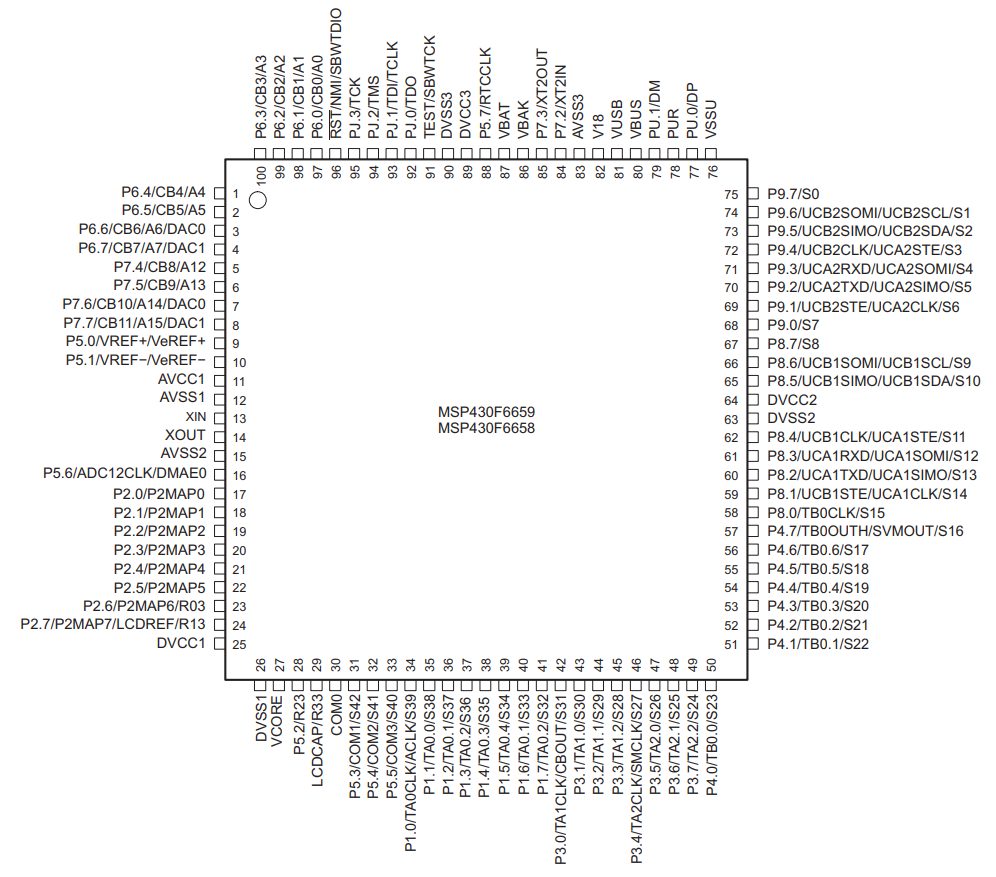
\includegraphics[width=0.9\textwidth]{figures/msp430-pinout.png}
        \caption{Microcontroller pinout positions.}
        \label{fig:msp430-pinout-positions}
    \end{center}
\end{figure}

\begin{longtable}{lcL{10cm}}
    \toprule[1.5pt]
    \textbf{Pin Code} & \textbf{Pin Number} & \textbf{Signal}       \\
    \midrule
    P1.0              & 34                  & MAIN\_RADIO\_ENABLE   \\
    P1.1              & 35                  & MAIN\_RADIO\_GPIO0    \\
    P1.2              & 36                  & MAIN\_RADIO\_GPIO1    \\
    P1.3              & 37                  & MAIN\_RADIO\_GPIO2    \\
    P1.4              & 38                  & MAIN\_RADIO\_RESET    \\
    P1.5              & 39                  & MAIN\_RADIO\_SPI\_CS  \\
    P1.6              & 40                  & TTC\_MCU\_SPI\_CS     \\
    P1.7              & 41                  & -                     \\
    \midrule
    P2.0              & 17                  & SPI\_CLK              \\
    P2.1              & 18                  & I2C0\_SDA             \\
    P2.2              & 19                  & I2C0\_SCL             \\
    P2.3              & 20                  & -                     \\
    P2.4              & 21                  & SPI\_MOSI             \\
    P2.5              & 22                  & SPI\_MISO             \\
    P2.6              & 23                  & -                     \\
    P2.7              & 24                  & -                     \\
    \midrule
    P3.0              & 42                  & I2C0\_EN              \\
    P3.1              & 43                  & I2C1\_EN              \\
    P3.2              & 44                  & I2C2\_EN              \\
    P3.3              & 45                  & I2C0\_READY           \\
    P3.4              & 46                  & I2C1\_READY           \\
    P3.5              & 47                  & I2C2\_READY           \\
    P3.6              & 48                  & PC104\_GPIO0          \\
    P3.7              & 49                  & PC104\_GPIO1          \\
    \midrule
    P4.0              & 50                  & PC104\_GPIO2          \\
    P4.1              & 51                  & PC104\_GPIO3          \\
    P4.2              & 52                  & MEM\_HOLD             \\
    P4.3              & 53                  & MEM\_RESET            \\
    P4.4              & 54                  & MEM\_SPI\_CS          \\
    P4.5              & 55                  & -                     \\
    P4.6              & 56                  & -                     \\
    P4.7              & 57                  & -                     \\
    \midrule
    P5.0              & 9                   & VREF                  \\
    P5.1              & 10                  & AGND                  \\
    P5.2              & 28                  & SYSTEM\_FAULT\_LED    \\
    P5.3              & 31                  & SYSTEM\_LED           \\
    P5.4              & 32                  & PAYLOAD\_0\_ENABLE    \\
    P5.5              & 33                  & PAYLOAD\_1\_ENABLE    \\
    P5.6              & 16                  & -                     \\
    P5.7              & 88                  & -                     \\
    \midrule
    P6.0              & 97                  & D\_BOARD\_ADC0        \\
    P6.1              & 98                  & D\_BOARD\_ADC1        \\
    P6.2              & 99                  & D\_BOARD\_ADC2        \\
    P6.3              & 100                 & OBDH\_CURRENT\_ADC    \\
    P6.4              & 1                   & OBDH\_VOLTAGE\_ADC    \\
    P6.5              & 2                   & D\_BOARD\_SPI\_CS0    \\
    P6.6              & 3                   & D\_BOARD\_SPI\_CS1    \\
    P6.7              & 4                   & -                     \\
    \midrule
    P7.0              & -                   & -                     \\
    P7.1              & -                   & -                     \\
    P7.2              & 84                  & XT2\_N                \\
    P7.3              & 85                  & XT2\_P                \\
    P7.4              & 5                   & D\_BOARD\_GPIO0       \\
    P7.5              & 6                   & D\_BOARD\_GPIO1       \\
    P7.6              & 7                   & D\_BOARD\_GPIO2       \\
    P7.7              & 8                   & D\_BOARD\_GPIO3       \\
    \midrule
    P8.0              & 58                  & -                     \\
    P8.1              & 59                  & -                     \\
    P8.2              & 60                  & UART1\_TX             \\
    P8.3              & 61                  & UART1\_RX             \\
    P8.4              & 62                  & -                     \\
    P8.5              & 65                  & I2C1\_SDA             \\
    P8.6              & 66                  & I2C1\_SCL             \\
    P8.7              & 67                  & ANTENNA\_GPIO         \\
    \midrule
    P9.0              & 68                  & -                     \\
    P9.1              & 69                  & FRAM\_SPI\_CS         \\
    P9.2              & 70                  & UART0\_TX             \\
    P9.3              & 71                  & UART0\_RX             \\
    P9.4              & 72                  & WDI\_EXT              \\
    P9.5              & 73                  & I2C2\_SDA             \\
    P9.6              & 74                  & I2C2\_SCL             \\
    P9.7              & 75                  & MR\_WDOG              \\
    \midrule
    PJ.0              & 92                  & TP21                  \\
    PJ.1              & 93                  & TP22                  \\
    PJ.2              & 94                  & TP23                  \\
    PJ.3              & 95                  & TP24                  \\
    \midrule
    -                 & 13                  & XT1IN                 \\
    -                 & 14                  & XT1OUT                \\
    -                 & 96                  & JTAG\_TDO\_TDI        \\
    -                 & 91                  & JTAG\_TCK             \\
    \bottomrule[1.5pt]
    \caption{Microcontroller pinout and assignments.}
    \label{tab:mcu-pinout}
\end{longtable}

\section{External Watchdog}

Additionally to the internal watchdog timer of the microcontroller, to ensure a system reset in case of a software freeze, an external watchdog circuit is being used. For that, the TPS3823 IC\nomenclature{\textbf{IC}}{\textit{Integrated Circuit.}} from Texas Instruments \cite{tps382x} was chosen. This IC is a voltage monitor with a watchdog timer feature. This circuit can be seen in the \autoref{fig:ext-wdt-circuit}.

This circuit works this way: if the WDI pin remains high or low longer than the timeout period, then reset is triggered. The timer clears when reset is asserted or when WDI sees a rising edge or a falling edge.

The watchdog timer task clears the TPS3823 timer by toggling the WDI pin at every $100\ ms$. If the WDI pin state stays unmodified for more than $1600\ ms$, the reset pin is cleared and the microcontroller is reseted.

\begin{figure}[!ht]
    \begin{center}
        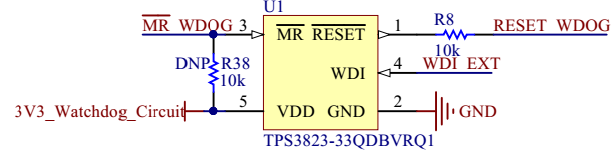
\includegraphics[width=0.65\textwidth]{figures/ext-watchdog-circuit.png}
        \caption{External watchdog timer circuit.}
        \label{fig:ext-wdt-circuit}
    \end{center}
\end{figure}

\section{Non-Volatile Memories}

There are two non-volatile memories available on the module: one flash NOR memory and one FRAM\nomenclature{\textbf{FRAM}}{\textit{Ferroelectric Random-Access Memory.}} memory.

\subsection{Flash NOR}

The flash NOR non-volatile memory model is the Micron MT25QL01GBBB, which is composed by a NOR flash architecture with 1 Gb of capacity (or 128 MB) and features extended SPI configurations. As can be seen in \autoref{fig:diagram-interfaces}, a SPI bus is used to communicate with this peripheral, using the \autoref{tab:usci-config} configurations. Also, there are some control pins that are connected to microcontroller GPIOs: HOLD\#, RESET\#, and W\#.

When RESET\# is driven LOW, the device is reset and the outputs are tri-stated. The HOLD\# signal pauses serial communications without deselecting or resetting the device, consequently outputs are tri-stated and inputs are ignored. The W\# signal handles as a write protection, which freezes the status register, turning its non-volatile bits read-only and preventing the write operation to be executed.


\begin{figure}[!ht]
    \begin{center}
        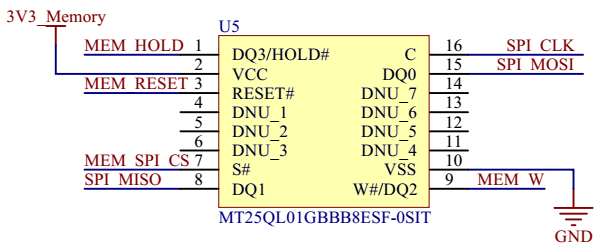
\includegraphics[width=0.65\textwidth]{figures/ext-memory-circuit.png}
        \caption{External memory circuit.}
        \label{fig:ext-mem-circuit}
    \end{center}
\end{figure}

\subsection{FRAM}

\begin{figure}[!ht]
    \begin{center}
        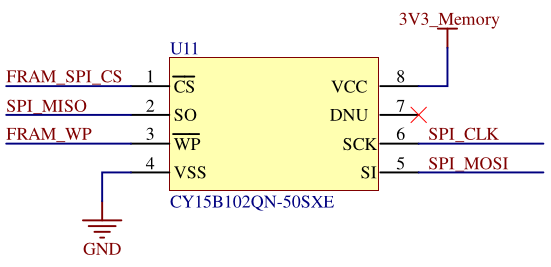
\includegraphics[width=0.65\textwidth]{figures/fram-memory-circuit.png}
        \caption{FRAM memory circuit.}
        \label{fig:fram-mem-circuit}
    \end{center}
\end{figure}

\section{I2C Buffers}

The microcontroller I2C interfaces have dedicated IC buffers, which improve the signal quality throughout the various connectors and offers reliability enhancements, since it protects the bus in case of failures. This measure was adopted in all the satellite modules due to previous failures in I2C buses. Using this scheme, the modules connected though this protocol might have shared connections without losing performance or reliability. 

The buffer selected for this function is the Texas Instruments TCA4311 device. Besides the I2C inputs and outputs, it features control and status signals that are connected to GPIOs in the microcontroller: an enable and an operation ready status. Also, both inputs and outputs in these I2C lines have external pull-up resistors.

\begin{figure}[!ht]
    \begin{center}
        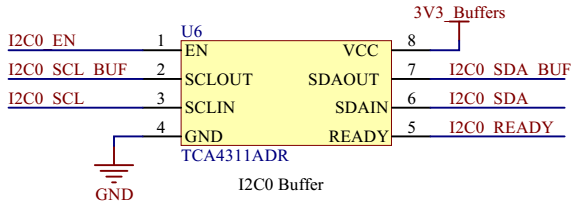
\includegraphics[width=0.65\textwidth]{figures/i2c-buffer-circuit.png}
        \caption{I2C buffer circuit.}
        \label{fig:i2c-buffer-circuit}
    \end{center}
\end{figure}

\section{RS-485 Transceiver}

The module features an RS-485 interface, which is connected to a 4H header (P8). This interface uses a transceiver (THVD1451) to convert the incoming RS-485 signals to UART and vice-versa. The outputs are $120\ \Omega$ differential pairs that have termination resistors before connecting to the header pins.

\begin{figure}[!ht]
    \begin{center}
        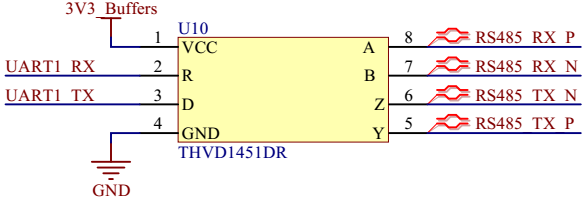
\includegraphics[width=0.65\textwidth]{figures/rs485-transceiver-circuit.png}
        \caption{RS-485 transceiver circuit.}
        \label{fig:rs485-transceiver-circuit}
    \end{center}
\end{figure}

\section{Voltage and Current Sensors}

In order to monitor the board overall current and voltage, the module have a current sensor using a Maxim Integrated IC (MAX9934) and a buffered voltage divider circuit with a Texas Instruments IC (TLV341A). These circuits have direct analog outputs that are connected to ADC inputs. The microcontroller internal ADC peripheral has a dedicated input for a voltage reference, which is connected to the REF5030A IC. This device generates a precise $3\ V$ output that enhances the measures and convertions performed by the microcontroller.

    %
% firmware.tex
%
% Copyright (C) 2021 by Universidade Federal de Santa Catarina.
%
% OBDH 2.0 Documentation
%
% This work is licensed under the Creative Commons Attribution-ShareAlike 4.0
% International License. To view a copy of this license,
% visit http://creativecommons.org/licenses/by-sa/4.0/.
%

%
% \brief Firmware chapter.
%
% \author Gabriel Mariano Marcelino <gabriel.mm8@gmail.com>
%
% \institution Universidade Federal de Santa Catarina (UFSC)
%
% \version 0.9.0
%
% \date 2019/10/30
%

\chapter{Firmware} \label{ch:firmware}

\section{Dependencies}

The firmware depends on external libraries to access the embedded hardware or to communicate with other modules. A list of these libraries and the used version is available in \autoref{tab:fw-dependencies}.

\begin{table}[!h]
    \centering
    \begin{tabular}{L{5cm}R{4cm}}
        \toprule[1.5pt]
        \textbf{Library}        & \textbf{Version} \\
        \midrule
            MSP430 DriverLib    & v2.91.11.01 \\
            FreeRTOS            & v10.2.1 \\
            NGHam protocol      & - \\
            libcsp              & v1.5.16 \\
        \bottomrule[1.5pt]
    \end{tabular}
    \caption{External libraries and dependencies of the firmware.}
    \label{tab:fw-dependencies}
\end{table}

\section{Tasks}

A list of the firmware tasks can be seen in the \autoref{tab:firmware-tasks}.

\begin{table}[!h]
    \centering
    \begin{tabular}{lccccc}
        \toprule[1.5pt]
        \textbf{Name}          & \textbf{Priority} & \textbf{Initial delay [ms]} & \textbf{Period [ms]} & \textbf{Stack [bytes]} \\
        \midrule
        Antenna deployment     & Highest & 0      & Aperiodic & 150  \\
        Antenna reading        & Medium  & 2000   & 60000     & 150  \\
        Beacon                 & High    & 1000   & 60000     & 1000 \\
        Data log               & Medium  & 2000   & 600000    & 225  \\
        EDC reading            & Medium  & 2000   & 60000     & 128  \\
        EPS reading            & Medium  & 2000   & 60000     & 384  \\
        Heartbeat              & Lowest  & 2000   & 500       & 160  \\
        Housekeeping           & Medium  & 2000   & 10000     & 160  \\
        Payload X reading      & Medium  & 5000   & 5000      & TBD  \\
        Radio periodoc reset   & High    & 60000  & 60000     & 128  \\
        Read sensors           & Medium  & 2000   & 60000     & 140  \\
        Startup (boot)         & Highest & 0      & Aperiodic & 350  \\
        System reset           & High    & 0      & 36000000  & 128  \\
        Telecommand processing & High    & 1000   & 5000      & 500  \\
        Time control           & Medium  & 1000   & 1000      & 128  \\
        TTC reading            & Medium  & 2000   & 60000     & 384  \\
        Uplink                 & Low     & 1000   & 10000     & 500  \\
        Watchdog reset         & Lowest  & 0      & 100       & 150  \\
        \bottomrule[1.5pt]
    \end{tabular}
    \caption{Firmware tasks.}
    \label{tab:firmware-tasks}
\end{table}

All these tasks are better described below.

\subsection{Antenna deployment}

.

\subsection{Antenna reading}

.

\subsection{Beacon}

.

\subsection{Data log}

This tasks saves the housekeeping data of the satellite in the flash memory at every 10 minutes.

\subsection{EDC reading}

.

\subsection{EPS reading}

.

\subsection{Heartbeat}

The heartbeat task keeps blinking a LED (``\textit{System LED}'' in \autoref{fig:status-leds}) at a rate of 1 Hz during the execution of the system. Its purpose is to give a visual feedback of the execution of the scheduler. This is tasks does not have a specific purpose on the flight version of the module (the flight version of the PCB does not have LEDs).

\subsection{Housekeeping}

.

\subsection{Payload X reading}

.

\subsection{Radio periodic reset}

.

\subsection{Read sensors}

This task reads the internal sensors of the OBDH at every 60 seconds.

\subsection{Startup (boot)}

This task is the first executed task when the system starts. All devices, libraries and data structures are initialized in this task. When the execution is done, the remaining tasks of the system are allowed to execute.

\subsection{System reset}

This task resets the microcontroller by software at every 10 hours. This can be useful to cleanup possible wrong values in variables, repeat the antenna deployment routine (limited to $n$ times), cleanup the RAM memory, etc.

\subsection{Telecommand processing}

.

\subsection{Time control}

This task is responsible for the time management of the system. At every second it increments the system time (epoch). Also, at every minute it saves the current system time in the non-volatile memory.

\subsection{TTC reading}

.

\subsection{Uplink}

.

\subsection{Watchdog reset}

This task resets the internal and external watchdog timer at every 100 ms. The internal watchdog has a maximum count time of 500 ms, and the external watchdog a maximum of 1600 ms (see \autoref{ch:hardware} for more information about the watchdog timers).

To prevent the system to not reset during an anomaly on some task (like an execution time longer than planned), this task has lowest possible priority: 0.

\section{Variables and Parameters}

The internal variables and parameters of the OBDH firmware can be seen in \autoref{tab:vars-and-pars}.

\begin{longtable}[c]{cL{0.82\textwidth}l}
    \toprule[1.5pt]
    \textbf{ID} & \textbf{Name/Description} & \textbf{Type}\\
    \midrule
    0   & Time counter in milliseconds                            & uint32 \\
    1   & Temperature of the $\mu$C in Kelvin                     & uint16 \\
    2   & Input current in mA                                     & uint16 \\
    3   & Input voltage in mV                                     & uint16 \\
    \multirow{18}{*}{4} & Last reset cause: & \multirow{18}{*}{uint8} \\
        & - 0x00 = No interrupt pending                           &        \\
        & - 0x02 = Brownout (BOR)                                 &        \\
        & - 0x04 = RST/NMI (BOR)                                  &        \\
        & - 0x06 = PMMSWBOR (BOR)                                 &        \\
        & - 0x08 = Wakeup from LPMx.5 (BOR)                       &        \\
        & - 0x0A = Security violation (BOR)                       &        \\
        & - 0x0C = SVSL (POR)                                     &        \\
        & - 0x0E = SVSH (POR)                                     &        \\
        & - 0x10 = SVML\_OVP (POR)                                &        \\
        & - 0x12 = SVMH\_OVP (POR)                                &        \\
        & - 0x14 = PMMSWPOR (POR)                                 &        \\
        & - 0x16 = WDT time out (PUC)                             &        \\
        & - 0x18 = WDT password violation (PUC)                   &        \\
        & - 0x1A = Flash password violation (PUC)                 &        \\
        & - 0x1C = Reserved                                       &        \\
        & - 0x1E = PERF peripheral/configuration area fetch (PUC) &        \\
        & - 0x20 = PMM password violation (PUC)                   &        \\
        & - 0x22 to 0x3E = Reserved                               &        \\
    5   & Reset counter                                           & uint16 \\
    6   & Last valid telecommand (uplink packet ID)               & uint8  \\
    7   & Temperature of the radio in Kelvin                      & uint16 \\
    8   & RSSI of the last valid telecommand                      & uint16 \\
    9   & Temperature of the antenna in Kelvin                    & uint16 \\
    \multirow{17}{*}{10} & Antenna status bits: & \multirow{17}{*}{uint16}  \\
        & - Bit 15: The antenna 1 is deployed (0) or not (1)      &        \\
        & - Bit 14: Cause of the latest activation stop for antenna 1 &    \\
        & - Bit 13: The antenna 1 deployment is active (1) or not (0) &    \\
        & - Bit 11: The antenna 2 is deployed (0) or not (1)      &        \\
        & - Bit 10: Cause of the latest activation stop for antenna 2 &    \\
        & - Bit 9: The antenna 2 deployment is active (1) or not (0)  &    \\
        & - Bit 8: The antenna is ignoring the deployment switches (1) or not (0) & \\
        & - Bit 7: The antenna 3 is deployed (0) or not (1)       &        \\
        & - Bit 6: Cause of the latest activation stop for antenna 3 &     \\
        & - Bit 5: The antenna 3 deployment is active (1) or not (0) &     \\
        & - Bit 4: The antenna system independent burn is active (1) or not (0) & \\
        & - Bit 3: The antenna 4 is deployed (0) or not (1)       &        \\
        & - Bit 2: Cause of the latest activation stop for antenna 4 &     \\
        & - Bit 1: The antenna 4 deployment is active (1) or not (0) &     \\
        & - Bit 0: The antenna system is armed (1) or not (0)     &        \\
    11  & Hardware version                                        & uint8 \\
    12  & Firmware version (ex.: ``v1.2.3'' = 0x00010203)         & uint32 \\
    13  & Mode (``Normal'' = 0, ``Hibernation'' = 1)              & uint8 \\
    14  & Timestamp of the last mode change                       & uint32 \\
    15  & Mode duration in sec. (valid only in hibernation mode)  & uint32 \\
    16  & Initial hibernation executed                            & boolean \\
    17  & Initial hibernation time counter (minutes)              & uint8 \\
    18  & Antenna deployment executed                             & boolean \\
    19  & Antenna deployment counter                              & uint8 \\
    \bottomrule[1.5pt]
    \caption{Variables and parameters of the OBDH 2.0.}
    \label{tab:vars-and-pars}
\end{longtable}

\section{Telemetry}


\subsection{Beacon}

The beacon packet is transmitted at every 1 minute and contains a basic telemetry data of the satellite. The content of this packet can be seen in \autoref{tab:telemetry-beacon}.

\begin{itemize}
    \item Period: 60 seconds
    \item Band: UHF
    \item Condition to operate: Always on
\end{itemize}

\begin{table}[!h]
    \centering
    \begin{tabular}{llc}
        \toprule[1.5pt]
        \textbf{Parameter} & \textbf{Content}       & \textbf{Length [bytes]} \\
        \midrule
        Packet ID          & 10h                    & 1 \\
        Satellite callsign & ``0PY0EGU''            & 7 \\
        $\mu$C temperature & Raw $\mu$C temperature & 2 \\
        $\mu$C voltage     & Raw $\mu$C voltage     & 2 \\
        $\mu$C current     & Raw $\mu$C current     & 2 \\
        Last reset cause   & Last reset cause ID    & 1 \\
        System time        & System time in ticks   & 4 \\
        Radio temperature  & Raw radio temperature  & 4 \\
        Last TC RSSI       & Raw RSSI value         & 2 \\
        Last received TC   & Last received TC ID    & 1 \\
        Battery 1 voltage  & Raw battery 1 voltage  & 2 \\
        Battery 2 voltage  & Raw battery 2 voltage  & 2 \\
        Battery current    & Raw battery current    & 2 \\
        Battery charge     & Raw battery charge     & 2 \\
        ...                & ...                    & ... \\
        \midrule
        Total              & -                      & 34 \\
        \bottomrule[1.5pt]
    \end{tabular}
    \caption{Beacon packet.}
    \label{tab:telemetry-beacon}
\end{table}

\subsection{EDC Information}

\begin{table}[!h]
    \centering
    \begin{tabular}{llc}
        \toprule[1.5pt]
        \textbf{Parameter} & \textbf{Content}                                 & \textbf{Len. [bytes]} \\
        \midrule
        Packet ID          & 11h                                              & 1 \\
        Satellite callsign & ``0PY0EGU''                                      & 7 \\
        \midrule
        \multicolumn{3}{c}{\textbf{PTT Decoder}} \\
        \midrule
        Time tag           & PTT signal receiving time                        & 4 \\
        Error code         & Error code                                       & 1 \\
        Carrier frequency  & Carrier frequency                                & 2 \\
        Carrier Abs        & Carrier amplitude at ADC interface output        & 2 \\
        Message length     & User message length in bytes                     & 1 \\
        User message       & ARGOS-2 PTT-A2 user message                      & 35 \\
        \midrule
        \multicolumn{3}{c}{\textbf{HK Info}} \\
        \midrule
        Current time       & Current time since J2000 epoch                   & 4 \\
        Elapsed time       & Elapsed time since last reset                    & 4 \\
        Current supply     & System current supply in mA                      & 2 \\
        Voltage supply     & System voltage supply in mV                      & 2 \\
        Temperature        & EDC board temperature                            & 1 \\
        PLL sync bit       & RF front end LO...                               & 1 \\
        ADC RMS            & RMS level at front-end output                    & 2 \\
        Num of RX PTT      & Generated PTT packages since last initialization & 1 \\
        Max                &                                                  & 1 \\
        Memory error count &                                                  & 1 \\
        \midrule
        \multicolumn{3}{c}{\textbf{System State}} \\
        \midrule
        Current time       &                                                  & 4 \\
        PTT available      & Number of PTT Package available for reading      & 1 \\
        PTT is paused      & PTT decoder task status                          & 1 \\
        Sampler state      & ADC sampler state                                & 1 \\
        \midrule
        Total              & -                                                & 79 \\
        \bottomrule[1.5pt]
    \end{tabular}
    \caption{EDC information packet.}
    \label{tab:telemetry-edc}
\end{table}

\subsection{EDC Samples}

The EDC samples are XX bytes long and are transmitted in Y packets with 219 bytes each

\begin{table}[!h]
    \centering
    \begin{tabular}{llc}
        \toprule[1.5pt]
        \textbf{Parameter} & \textbf{Content}               & \textbf{Length [bytes]} \\
        \midrule
        Packet ID          & 12h                            & 1 \\
        Satellite callsign & ``0PY0EGU''                    & 7 \\
        Time tag           & Elapsed time since J2000 epoch & 4 \\
        Packet counter     & ADC sample packet number       & 1 \\
        I sample[n]        & First ADC I-sample             & 2 \\
        Q sample[n]        & First ADC Q-sample             & 2 \\
        ...                & ...                            & ... \\
        I sample[n+102]    & First ADC I-sample             & 2 \\
        Q sample[n+102]    & First ADC Q-sample             & 2 \\
        \midrule
        Total              & -                              & 219 \\
        \bottomrule[1.5pt]
    \end{tabular}
    \caption{EDC samples packet.}
    \label{tab:telemetry-edc-samples}
\end{table}

\section{Telecommands}

\begin{table}[!h]
    \centering
    \begin{tabular}{lll}
        \toprule[1.5pt]
        \textbf{Name}          & \textbf{Parameters}           & \textbf{Access} \\
        \midrule
        Enter hibernation      & Hibernation period in seconds & Private         \\
        Leave hibernation      & None                          & Private         \\
        Activate beacon        & None                          & Private         \\
        Deactivate beacon      & None                          & Private         \\
        Activate downlink      & None                          & Private         \\
        Deactivate downlink    & None                          & Private         \\
        Activate EDC           & None                          & Private         \\
        Deactivate EDC         & None                          & Private         \\
        Get EDC info           & None                          & Private         \\
        Activate Payload X     & Experiment period in seconds  & Private         \\
        Deactivate Payload X   & None                          & Private         \\
        Set system time        & Time value (epoch)            & Private         \\
        Ping                   & None                          & Public          \\
        Message broadcast      & ASCII message                 & Public          \\
        Request data           & Data flags                    & Public          \\
        \bottomrule[1.5pt]
    \end{tabular}
    \caption{System telecomamnds.}
    \label{tab:system-telecommands}
\end{table}

\subsection{Enter hibernation}

\begin{table}[!h]
    \centering
    \begin{tabular}{lll}
        \toprule[1.5pt]
        \textbf{Parameter}      & \textbf{Content}                         & \textbf{Length [bytes]} \\
        \midrule
        Packet ID               & 20h                                      & 1 \\
        Ground station callsign & Any callsign (ASCII, filled with ``0''s) & 7 \\
        Hibernation period      & Period in minutes (1 to 65535)           & 2 \\
        Key                     & Telecommand key (ASCII)                  & 10 \\
        \midrule
        Total                   & -                                        & 20 \\
        \bottomrule[1.5pt]
    \end{tabular}
    \caption{Enter hibernation telecommand.}
    \label{tab:enter-hibernation-tc}
\end{table}

\subsection{Leave hibernation}

\begin{table}[!h]
    \centering
    \begin{tabular}{lll}
        \toprule[1.5pt]
        \textbf{Parameter}      & \textbf{Content}                         & \textbf{Length [bytes]} \\
        \midrule
        Packet ID               & 21h                                      & 1 \\
        Ground station callsign & Any callsign (ASCII, filled with ``0''s) & 7 \\
        Key                     & Telecommand key (ASCII)                  & 10 \\
        \midrule
        Total                   & -                                        & 18 \\
        \bottomrule[1.5pt]
    \end{tabular}
    \caption{Leave hibernation telecommand.}
    \label{tab:leave-hibernation-tc}
\end{table}

\subsection{Activate beacon}

.

\subsection{Deactivate beacon}

.

\subsection{Activate EDC}

.

\subsection{Deactivate EDC}

.

\subsection{Get EDC info}

This telecommand request information from the EDC payload. When received, the OBDH transmits the housekeeping and state frames of the EDC module (28 bytes). This telecommand does not requires a key.

\subsection{Activate Payload X}

.

\subsection{Deactivate Payload X}

.

\subsection{Set system time}

.

\subsection{Ping}

\begin{table}[!h]
    \centering
    \begin{tabular}{lll}
        \toprule[1.5pt]
        \textbf{Parameter}      & \textbf{Content}                         & \textbf{Length [bytes]} \\
        \midrule
        Packet ID               & 22h                                      & 1 \\
        Ground station callsign & Any callsign (ASCII, filled with ``0''s) & 7 \\
        \midrule
        Total                   & -                                        & 8 \\
        \bottomrule[1.5pt]
    \end{tabular}
    \caption{Ping telecommand.}
    \label{tab:ping-tc}
\end{table}

\begin{table}[!h]
    \centering
    \begin{tabular}{lll}
        \toprule[1.5pt]
        \textbf{Parameter}      & \textbf{Content}                               & \textbf{Length [bytes]} \\
        \midrule
        Packet ID               & 12h                                            & 1 \\
        Satellite callsign      & ``PY0EGU''                                     & 7 \\
        Destination callsign    & Requester callsign (ASCII, filled with ``0''s) & 7 \\
        \midrule
        Total                   & -                                              & 15 \\
        \bottomrule[1.5pt]
    \end{tabular}
    \caption{Ping telecommand answer.}
    \label{tab:ping-tc-ans}
\end{table}

\subsection{Message broadcast}

\begin{table}[!h]
    \centering
    \begin{tabular}{lll}
        \toprule[1.5pt]
        \textbf{Parameter}      & \textbf{Content}                         & \textbf{Length [bytes]} \\
        \midrule
        Packet ID               & 23h                                      & 1 \\
        Ground station callsign & Any callsign (ASCII, filled with ``0''s) & 7 \\
        Message                 & Message to broadcast (ASCII)             & up to  \\
        \midrule
        Total                   & -                                        & 8 \\
        \bottomrule[1.5pt]
    \end{tabular}
    \caption{Message broadcast telecommand.}
    \label{tab:msg-broadcast-tc}
\end{table}

\subsection{Request data}

.

\section{Operating System}

As operating system the FreeRTOS 10 \cite{freertos} is being used. FreeRTOS is a market-leading real-time operating system (RTOS) for microcontrollers and small microprocessors. Distributed freely under the MIT open source license, FreeRTOS includes a kernel and a growing set of IoT libraries suitable for use across all industry sectors. FreeRTOS is built with an emphasis on reliability and ease of use.

The main configuration parameters of the operating system in this project are availabe in \autoref{tab:freertos-config}.

\begin{table}[!h]
    \centering
    \begin{tabular}{lrr}
        \toprule[1.5pt]
        \textbf{Parameter}       & \textbf{Value} & \textbf{Unit} \\
        \midrule
        Version                  & v10.2.0        & - \\
        Tick rate (Hz)           & 1000           & Hz \\
        CPU clock (HZ)           & 32             & MHz \\
        Max. priorities          & 5              & - \\
        Heap size                & 40960          & bytes \\
        Max. length of task name & 20             & - \\
        \bottomrule[1.5pt]
    \end{tabular}
    \caption{FreeRTOS main configuration parameters.}
    \label{tab:freertos-config}
\end{table}

More details of the used configuration parameters can be seen in the file \textit{\href{https://github.com/spacelab-ufsc/obdh2/blob/master/firmware/config/FreeRTOSConfig.h}{firmware/config/FreeRTOSConfig.h}} from \cite{obdh2-repo}.

\section{Hardware Abstraction Layer (HAL)}

As the Hardware Abstraction Layer (HAL\nomenclature{\textbf{HAL}}{\textit{Hardware Abstraction Layer.}}), the DriverLib \cite{driverlib} from Texas Instruments is begin used. It is the official API to access the registers of the MSP430 microcontrollers.

The DriverLib is meant to provide a ``software'' layer to the programmer in order to facilitate higher level of programming compared to direct register accesses. By using the high level software APIs provided by DriverLib, users can create powerful and intuitive code which is highly portable between not only devices within the MSP430 platform, but between different families in the MSP430/MSP432 platforms.

\section{Memory Management}

.

\section{Protocols}

\subsection{NGHam}

NGHam \cite{ngham}, short for Next Generation Ham Radio, is a set of protocols for packet radio communication. Its usage is similar to the existing AX.25 protocol.

\begin{figure}[!ht]
    \begin{center}
        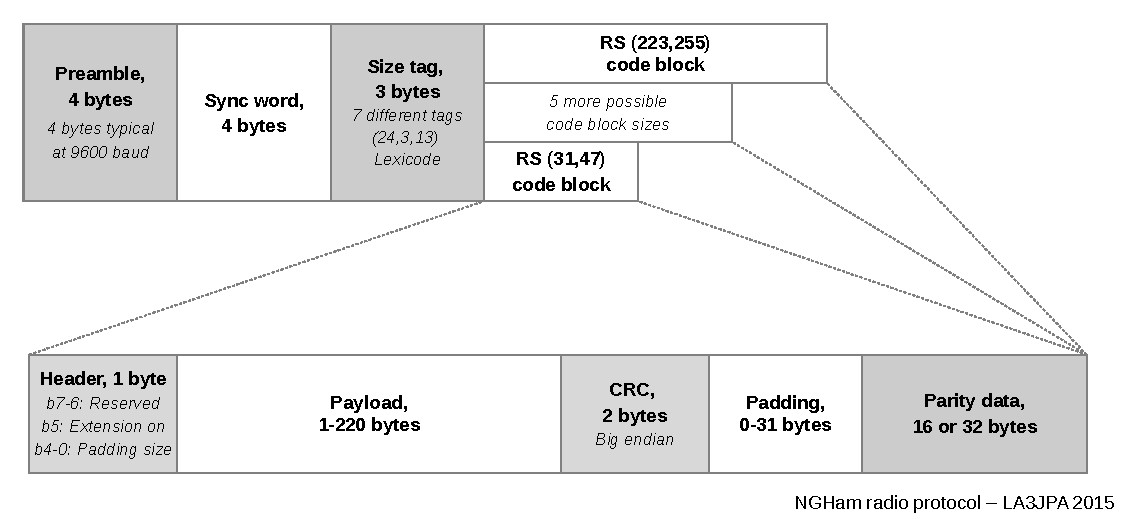
\includegraphics[width=\textwidth]{figures/ngham_block_v4.pdf}
        \caption{NGHam packet structure.}
        \label{fig:ngham-stack}
    \end{center}
\end{figure}

\subsection{CSP}

The CubeSat Space Protocol (CSP) \cite{csp} is a small protocol stack written in C. CSP is designed to ease communication between distributed embedded systems in smaller networks, such as CubeSats. The design follows the TCP/IP model and includes a transport protocol, a routing protocol and several MAC-layer interfaces. The core of libcsp includes a router, a connection oriented socket API and message/connection pools.

The idea is to give sub-system developers of CubeSats the same features of a TCP/IP stack, but without adding the huge overhead of the IP header. The small footprint and simple implementation allows a small 8-bit system to be fully connected on the network. This allows all subsystems to provide their services on the same network level, without any master node required. Using a service oriented architecture has several advantages compared to the traditional mater/slave topology used on many cubesats.

The OBDH's firmware currently uses the version \href{https://github.com/GomSpace/libcsp/releases/tag/1.5.16}{v1.5.16} of the libcsp library.

    %
% assembly.tex
%
% Copyright (C) 2021 by Universidade Federal de Santa Catarina.
%
% OBDH 2.0 Documentation
%
% This work is licensed under the Creative Commons Attribution-ShareAlike 4.0
% International License. To view a copy of this license,
% visit http://creativecommons.org/licenses/by-sa/4.0/.
%

%
% \brief Assembly instructions chapter.
%
% \author Gabriel Mariano Marcelino <gabriel.mm8@gmail.com>
%
% \institution Universidade Federal de Santa Catarina (UFSC)
%
% \version 0.7.0
%
% \date 2020/05/12
%

\chapter{Board Assembly} \label{ch:assembly}

The OBDH2 has some DNP components to provide flashing, debugging, testing or providing extra interfaces if needed. These components may not be necessary for the flight model of the board. The draftsman document can be viewed for more detailed information regarding their location and board dimensions \cite{obdh2-draftsman}.

\section{Development Model}

\subsection{Debug and programming connectors}

The P2 and P6 connectors are used for flashing and debugging the OBDH2 board. \hyperref[sec:programer-and-debug]{See again chapter 3 (Hardware) and subsection 3.2.3 (Programmer and Debug) for more information}.

\subsection{Status leds}

As already exposed before in the document OBDH2 has status leds to be used during development and test phases. \hyperref[sec:status-leds]{See again chapter 2 (System Overview) and the subsection 2.3.1 (Status Leds) for more information}.

\subsection{Analog circuits}

TBD

\section{Flight Model}

TBD

\section{Custom Configuration}

On the PC104 connector of OBDH2 there are some jumper resistors to enable extra I2C, SPI and GPIOs interfaces if desired. Note that the I2C0, I2C1 and SPI channels should not be used with shared devices. The corresponding table and location on the pcb of these components are showed below. 

\begin{table}[!h]
    \centering
    \begin{tabular}{cllll}
        \toprule[1.5pt]
        \textbf{Label} & \textbf{Interface} \\
        \midrule
        J\_PC1            & I2C0\_SDA \\
        J\_PC2            & I2C0\_SCL \\
        J\_PC3            & I2C1\_SDA \\
        J\_PC4            & I2C1\_SCL \\
        J\_PC5            & SPI\_MOSI \\
        J\_PC6            & SPI\_MISO \\
        J\_PC7            & SPI\_CLK \\
        J\_PC8            & GPI0 \\
        J\_PC9            & GPIO1 \\
        J\_PC10           & GPIO2 \\
        J\_PC11           & GPIO3 \\
        \bottomrule[1.5pt]
    \end{tabular}
    \caption{Additional PC104 inferfaces.}
    \label{tab:additional-pc104-inferfaces}
\end{table}

\begin{figure}[!ht]
    \begin{center}
         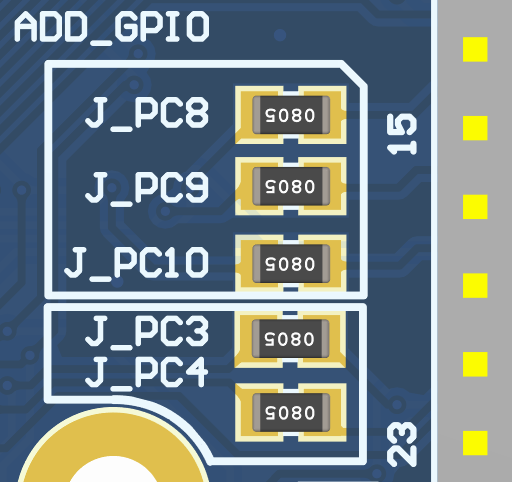
\includegraphics[width=55mm]{figures/add_gpio_i2c1_jumpers.png}
        \caption{Additional GPIOs and I2C channel 1.}
        \label{fig:add_gpio_i2c1_jumpers}
        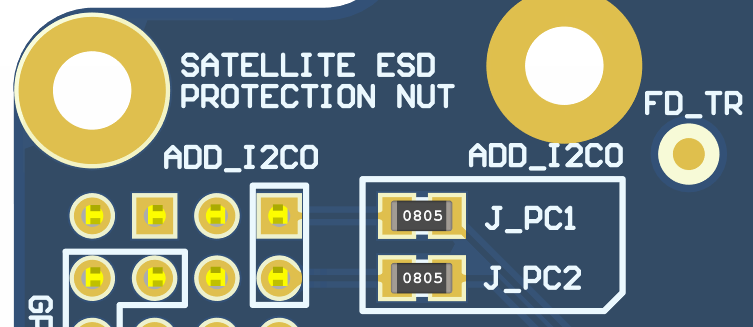
\includegraphics[width=90mm]{figures/add_i2c0_jumpers.png}
        \caption{Additional I2C channel 0.}
        \label{fig:add_i2c0_jumpers}
        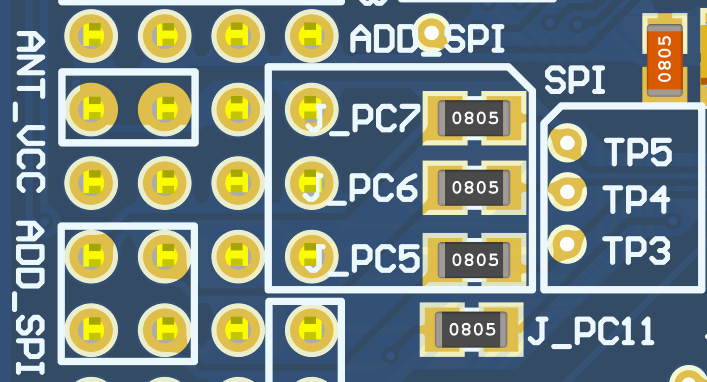
\includegraphics[width=80mm]{figures/add_spi_1gpio_jumpers.png}
        \caption{Additional GPIO and SPI channel.}
        \label{fig:add_spi_1gpio_jumpers}
    \end{center}
\end{figure}

    %
% introduction.tex
%
% Copyright (C) 2020 by Universidade Federal de Santa Catarina.
%
% OBDH 2.0 Documentation
%
% This work is licensed under the Creative Commons Attribution-ShareAlike 4.0
% International License. To view a copy of this license,
% visit http://creativecommons.org/licenses/by-sa/4.0/.
%

%
% \brief Instructions chapter.
%
% \author Gabriel Mariano Marcelino <gabriel.mm8@gmail.com>
% \author André Martins Pio de Mattos <andrempmattos@gmail.com>
%
% \institution Universidade Federal de Santa Catarina (UFSC)
%
% \version 0.10.0
%
% \date 07/05/2020
%

\chapter{Usage Instructions} \label{ch:instructions}

\section{Powering the Board}

Since the OBDH 2.0 is a service module within a satellite bus, to correctly provide its power supply, it requires an external $3.3\pm0.2\ V$ power input and a current capability of at least $100\ mA$ (might change depending on the daughterboard requirements). As presented in the PC-104 and programming interface sections, some options are given to power the module to improve flexibility during development. The board has two power schemes: the JTAG interface for debugging, and the PC-104, for the flight configuration. The first case uses both P1 or P2 connectors as power input (besides the JTAG and UART interfaces) and requires a jumper connection in the P6 connector. The second uses the PC-104 pins H1-45 and H1-46 to provide the power, and the P6 connector should remain open. For pinout details, refer to the external connectors in the hardware chapter.

\section{Log Messages}

The OBDH 2.0 has a UART interface dedicated to debugging, described in \autoref{tab:usci-config}. It follows a log system structure to improve the information provided in each message. The \autoref{fig:putty-output} shows an example of the logging system, more specifically the initialization sequence. The messages use the following scheme: in green inside brackets, the timestamp; in magenta, the scope (or origin) of the log; and lastly the actual message, which might be white (info or note), yellow (warning), and red (error).

\begin{figure}[!ht]
    \begin{center}
        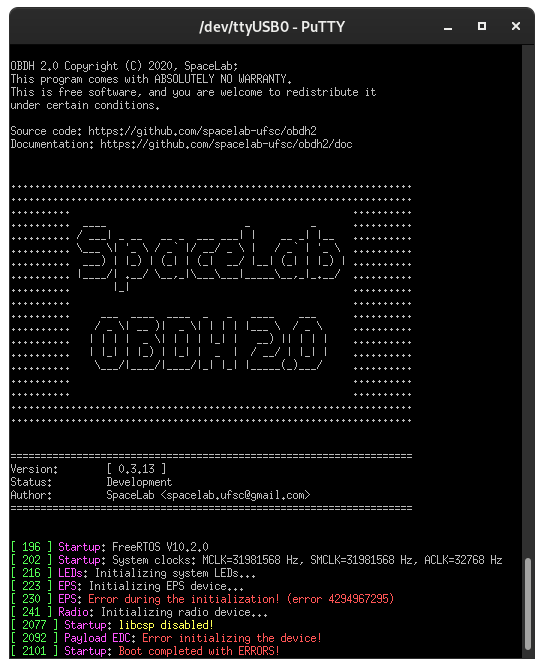
\includegraphics[width=0.75\textwidth]{figures/putty-output.png}
        \caption{Firmware initialization on PuTTy.}
        \label{fig:putty-output}
    \end{center}
\end{figure}

\section{Daughterboards Installation}

The daughterboard requirements might change for each application board attached. Then, it is important to check at least a minimal set of mandatory characteristics. First, it is important to verify mechanical parameters that concern size (recommended $63.5 \times 43.5\ mm$), maximum height (no higher than $7\ mm$), screw attachment (refer to mechanical sheet \cite{obdh2-draftsman}), and contact connector positioning. After this, the electrical interface must be checked (refer to \autoref{sec:daughterboard-interface}). There are 3 different power supply options, a $3.3\ V$ source shared with the OBDH board itself, another $3.3\ V$ source shared with the antenna deployer, and the main battery bus that ranges from $5.4$ to $8.4\ V$. Lastly, depending on the application board design, it is necessary to check communication interface protocols and parameters, control inputs and outputs, and external interfaces with other modules.

    %
% introduction.tex
%
% Copyright (C) 2020 by Universidade Federal de Santa Catarina.
%
% OBDH 2.0 Documentation
%
% This work is licensed under the Creative Commons Attribution-ShareAlike 4.0
% International License. To view a copy of this license,
% visit http://creativecommons.org/licenses/by-sa/4.0/.
%

%
% \brief References chapter.
%
% \author Gabriel Mariano Marcelino <gabriel.mm8@gmail.com>
%
% \institution Universidade Federal de Santa Catarina (UFSC)
%
% \version 0.5.0
%
% \date 2019/07/18
%

\bibliography{references/ngham,%
              references/reliance_edge,%
              references/msp430f6659,%
              references/fsi-conn,%
              references/tps382x,%
              references/obdh2-repo,%
              references/freertos,%
              references/csp,%
              references/driverlib,%
              references/obdh2-draftsman,%
              references/floripasat2,%
              references/obdh-fsat}

\addcontentsline{toc}{chapter}{References}

    %
% appendices.tex
%
% Copyright (C) 2021 by SpaceLab.
%
% OBDH 2.0 Documentation
%
% This work is licensed under the Creative Commons Attribution-ShareAlike 4.0
% International License. To view a copy of this license,
% visit http://creativecommons.org/licenses/by-sa/4.0/.
%

%
% \brief Appendices.
%
% \author Gabriel Mariano Marcelino <gabriel.mm8@gmail.com>
%
% \institution Universidade Federal de Santa Catarina (UFSC)
%
% \version 0.6.0
%
% \date 2021/04/17
%

\begin{appendices}

%
% test_report_v05.tex
%
% Copyright (C) 2021 by SpaceLab.
%
% OBDH 2.0 Documentation
%
% This work is licensed under the Creative Commons Attribution-ShareAlike 4.0
% International License. To view a copy of this license,
% visit http://creativecommons.org/licenses/by-sa/4.0/.
%

%
% \brief Test report of the v0.5 hardware.
%
% \author Gabriel Mariano Marcelino <gabriel.mm8@gmail.com>
%
% \institution Universidade Federal de Santa Catarina (UFSC)
%
% \version 0.6.0
%
% \date 2021/04/17
%

\chapter{Test Report of v0.5 Version} \label{anx:test-report-v05}

This appendix is a test report of the first manufactured and assembled PCB (version v0.5).

\begin{itemize}
    \item \textbf{PCB manufacturer}: PCBWay (China)
    \item \textbf{PCB assembly}: PCBWay (China)
    \item \textbf{PCB arrival date}: 2021/04/14
    \item \textbf{Execution date}: 2021/04/16 to \textcolor{red}{TBC}
    \item \textbf{Tester}: G. M. Marcelino
\end{itemize}

\section{Visual Inspection}

\begin{itemize}
    \item \textbf{Test description/Objective}: Inspection of the board, visually and with a multimeter, searching for fabrication and assembly failures.
    \item \textbf{Material}:
        \begin{itemize}
            \item Multimeter UNI-T DT830B
        \end{itemize}
    \item \textbf{Results}: The results of this test can be seen in Figures \ref{fig:obdh2-v05-top} (top view of the board) and \ref{fig:obdh2-v05-bottom} (bottom view of the board).
    \item \textbf{Conclusion}: No problems were identified on this test.
\end{itemize}

\begin{figure}[!ht]
    \begin{center}
        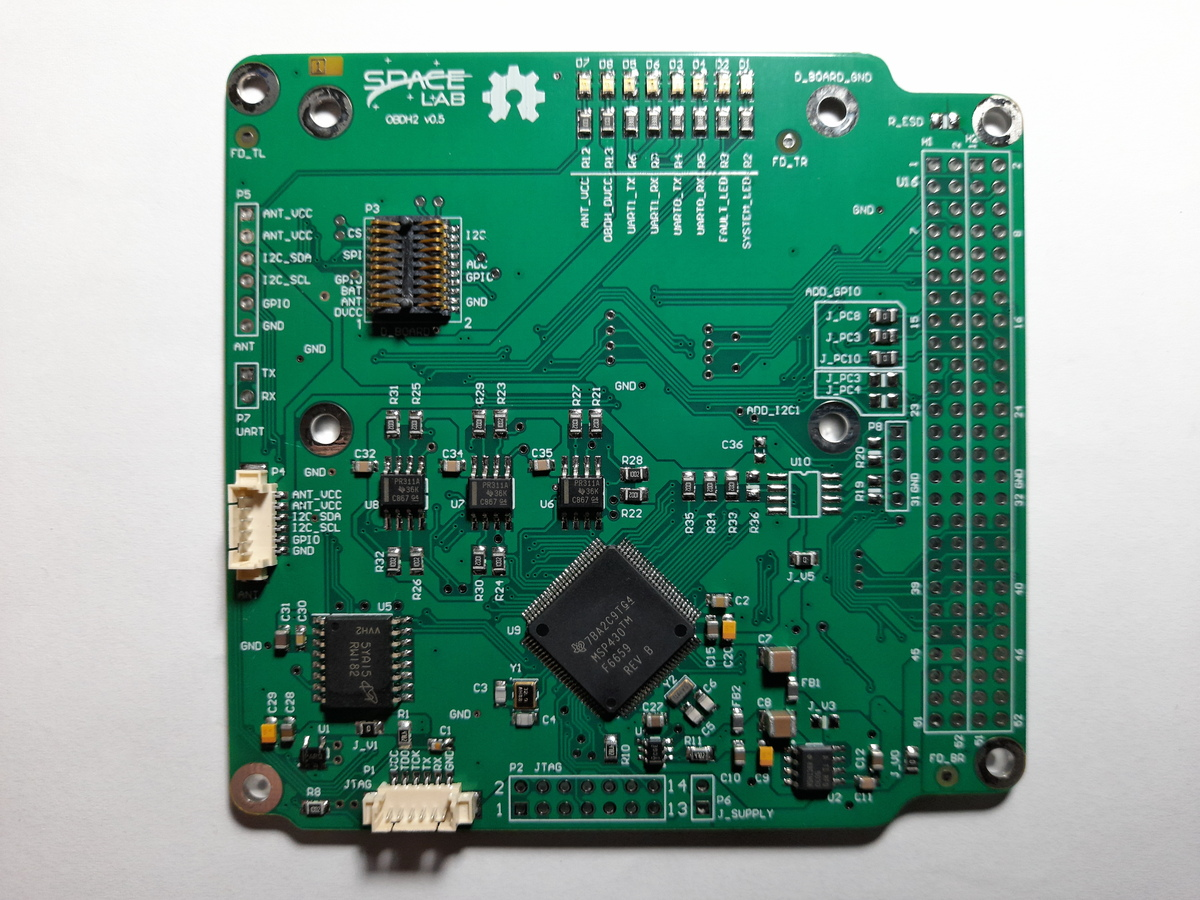
\includegraphics[width=\columnwidth]{figures/v05/obdh2-v05-top.jpg}
        \caption{Top view of the OBDH 2.0 v0.5 board.}
        \label{fig:obdh2-v05-top}
    \end{center}
\end{figure}

\begin{figure}[!ht]
    \begin{center}
        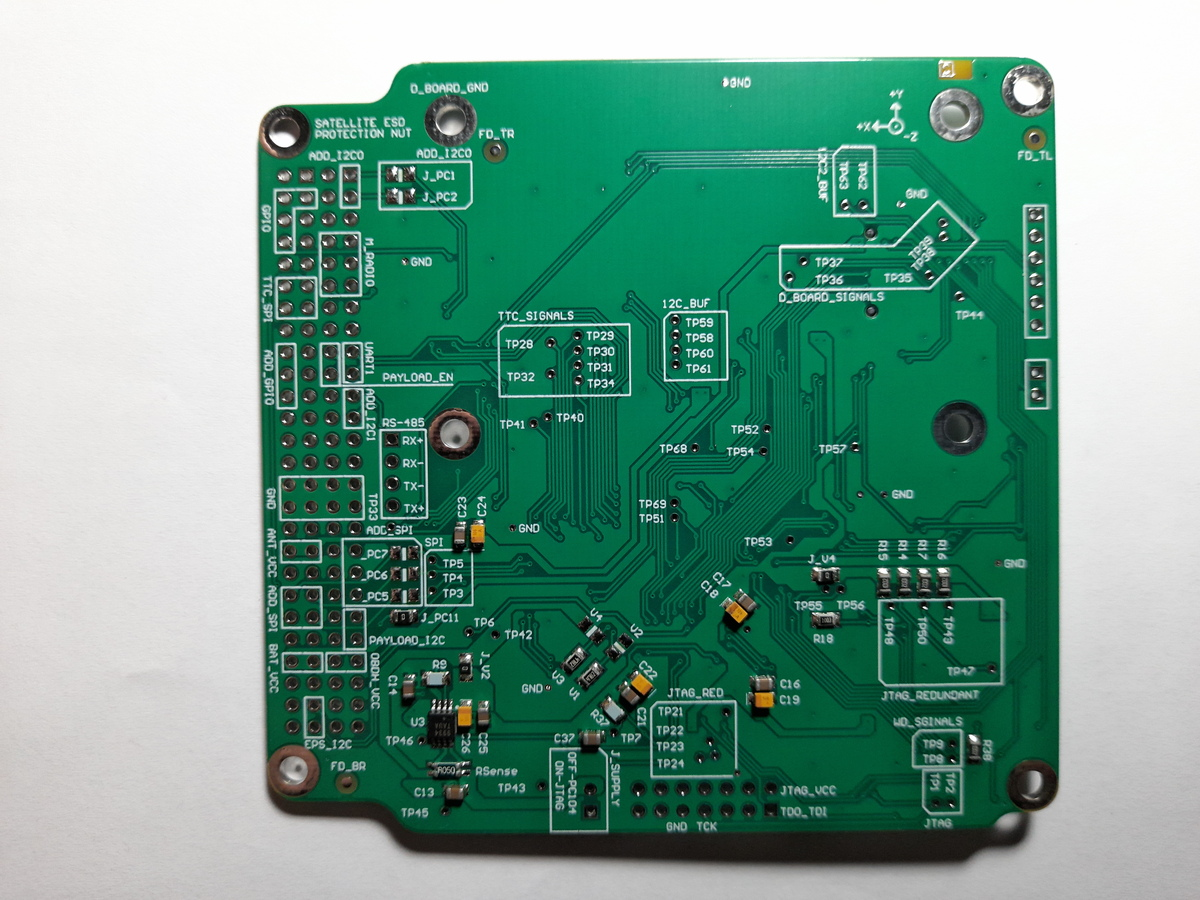
\includegraphics[width=\columnwidth]{figures/v05/obdh2-v05-bottom.jpg}
        \caption{Bottom view of the OBDH 2.0 v0.5 board.}
        \label{fig:obdh2-v05-bottom}
    \end{center}
\end{figure}

\section{Firmware Programming}

\begin{itemize}
    \item \textbf{Test description/Objective}: Inspection of the board, visually and with a multimeter, searching for fabrication and assembly mistakes.
    \item \textbf{Material}:
        \begin{itemize}
            \item Code Composer Studio v9.3.0
            \item MSP-FET Flash Emulation Tool
            \item USB-UART converter
            \item Screen (Linux software)
        \end{itemize}
    \item \textbf{Results}: The results of this are available in \autoref{fig:log-first-boot}, where the log messages of the first boot of the board can be seen.
    \item \textbf{Conclusion}: No problems were identified on this test.
\end{itemize}

\begin{figure}[!ht]
    \begin{center}
        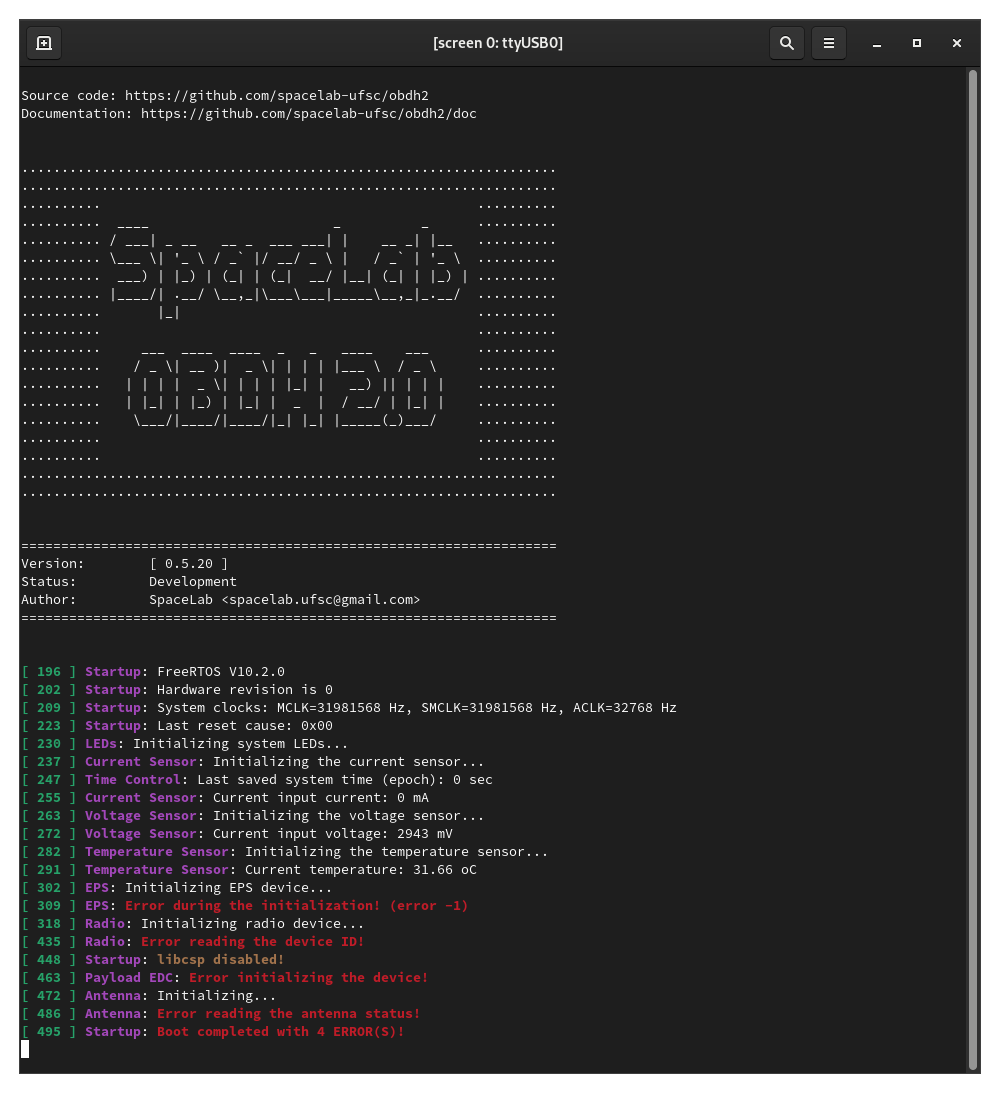
\includegraphics[width=0.7\columnwidth]{figures/v05/log-first-boot.png}
        \caption{Log messages during the first boot.}
        \label{fig:log-first-boot}
    \end{center}
\end{figure}

\section{Communication Busses}

\begin{itemize}
    \item \textbf{Test description/Objective}: Test the communication busses of the board, as listed below:
        \begin{itemize}
            \item I$^{2}$C Port 0
            \item I$^{2}$C Port 1
            \item I$^{2}$C Port 2
        \end{itemize}
    \item \textbf{Material}:
        \begin{itemize}
            \item Saleae Logic Analyzer (24 MHz, 8 channels)
            \item Saleae Logic software (v1.2.18)
            \item MSP-FET Flash Emulation Tool
        \end{itemize}
    \item \textbf{Results}: The results of this test can be seen in Figures \ref{fig:test-i2c-0}, \ref{fig:test-i2c-1} and \ref{fig:test-i2c-2}.
    \item \textbf{Conclusion:} No problems were identified on this test, all buses are working as expected.
\end{itemize}

\begin{figure}[!htb]
    \begin{center}
        \subfigure[Connections of the I$^{2}$C port 0 test.\label{fig:connections-i2c-0}]{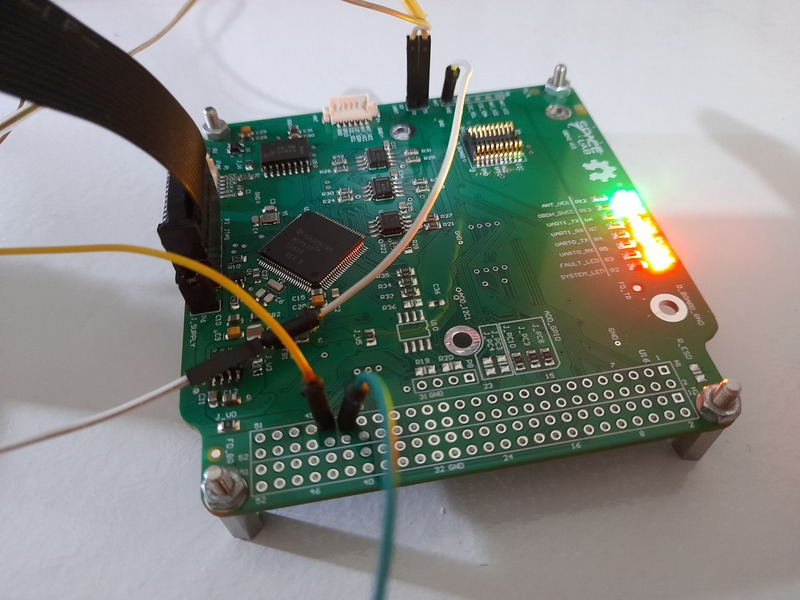
\includegraphics[height=0.22\textheight]{figures/v05/test-i2c-0.jpg}}
        ~
        \subfigure[Waveforms of the I$^{2}$C port 0 test.\label{fig:waveform-i2c-0}]{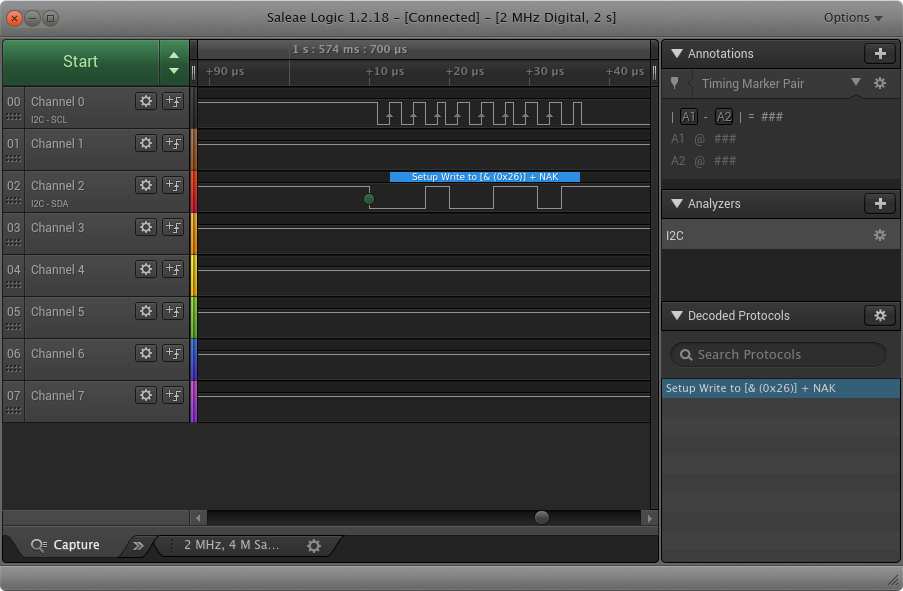
\includegraphics[height=0.22\textheight]{figures/v05/waveform-i2c-0.png}}
        \caption{I$^{2}$C port 0 test.}
        \label{fig:test-i2c-0}
    \end{center}
\end{figure}

%\begin{figure}[!ht]
%    \begin{center}
%        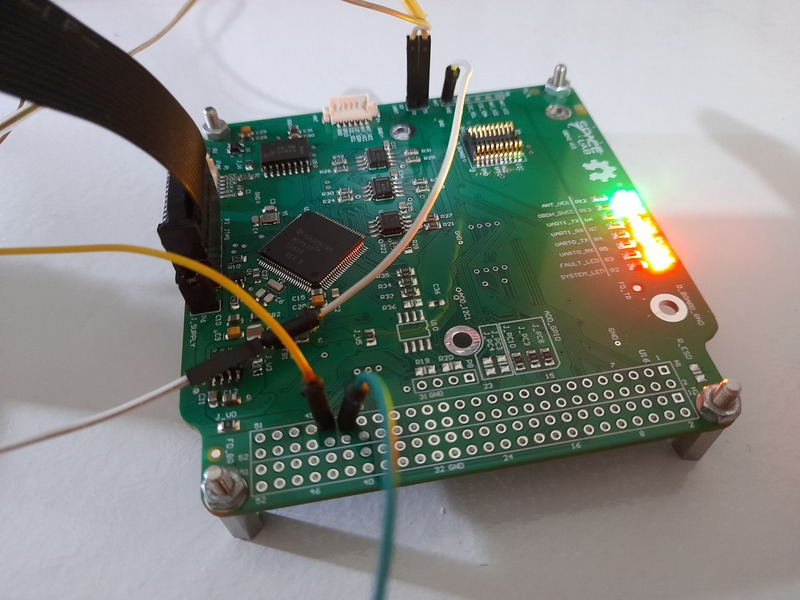
\includegraphics[width=0.7\columnwidth]{figures/v05/test-i2c-0.jpg}
%        \caption{Connections of the I2C port 0 test.}
%        \label{fig:test-i2c-0}
%    \end{center}
%\end{figure}
%
%\begin{figure}[!ht]
%    \begin{center}
%        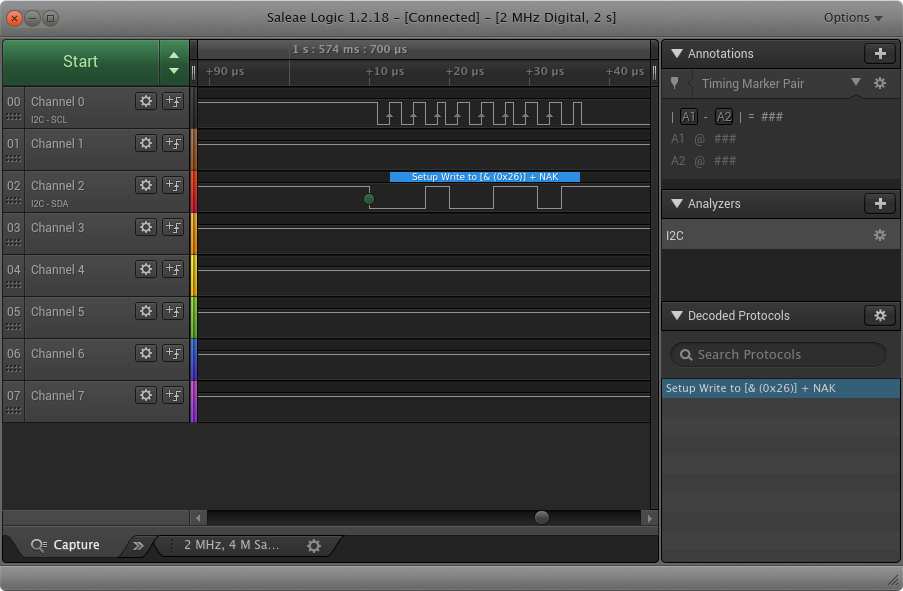
\includegraphics[width=\columnwidth]{figures/v05/waveform-i2c-0.png}
%        \caption{Waveform of the I2C port 0.}
%        \label{fig:waveform-i2c-0}
%    \end{center}
%\end{figure}

\begin{figure}[!htb]
    \begin{center}
        \subfigure[Connections of the I$^{2}$C port 1 test.\label{fig:connections-i2c-1}]{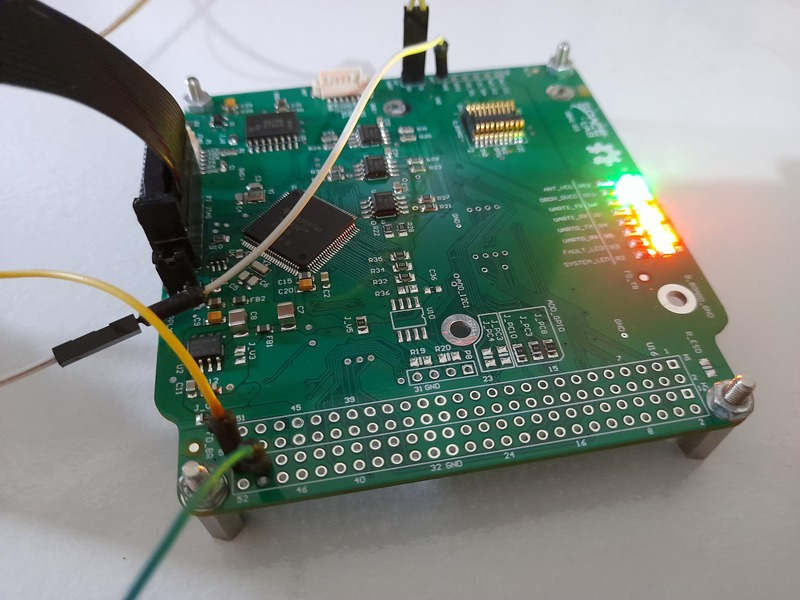
\includegraphics[height=0.22\textheight]{figures/v05/test-i2c-1.jpg}}
        ~
        \subfigure[Waveforms of the I$^{2}$C port 1 test.\label{fig:waveform-i2c-1}]{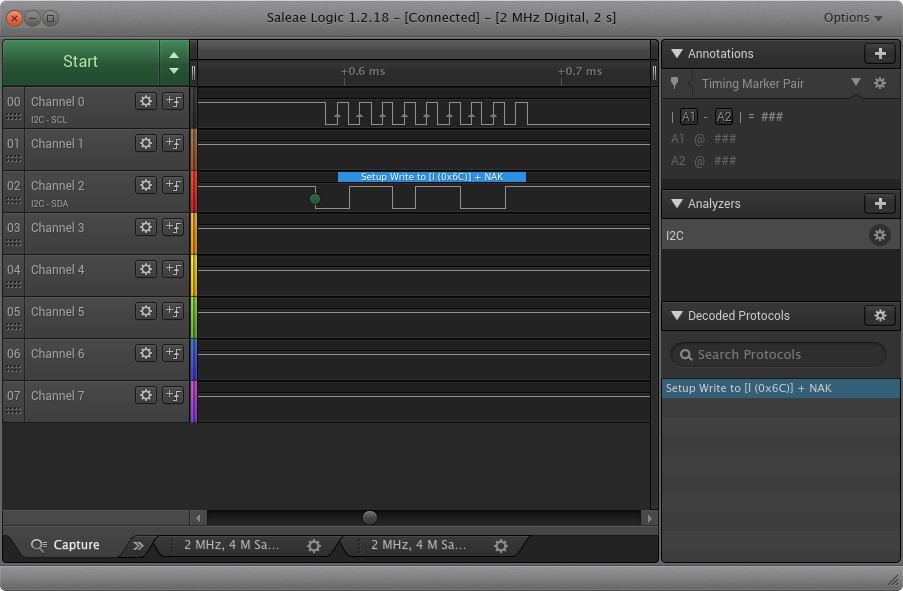
\includegraphics[height=0.22\textheight]{figures/v05/waveform-i2c-1.png}}
        \caption{I$^{2}$C port 1 test.}
        \label{fig:test-i2c-1}
    \end{center}
\end{figure}

%\begin{figure}[!ht]
%    \begin{center}
%        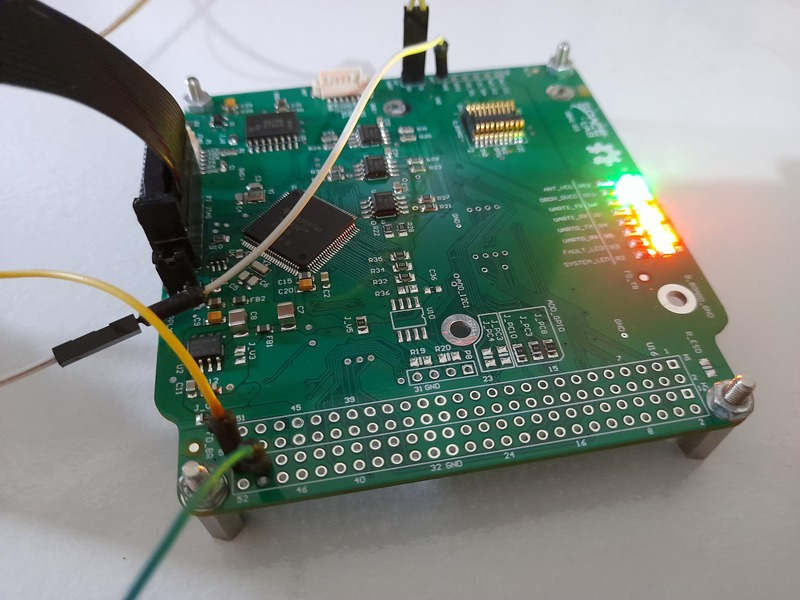
\includegraphics[width=0.7\columnwidth]{figures/v05/test-i2c-1.jpg}
%        \caption{Connections of the I2C port 1 test.}
%        \label{fig:test-i2c-1}
%    \end{center}
%\end{figure}
%
%\begin{figure}[!ht]
%    \begin{center}
%        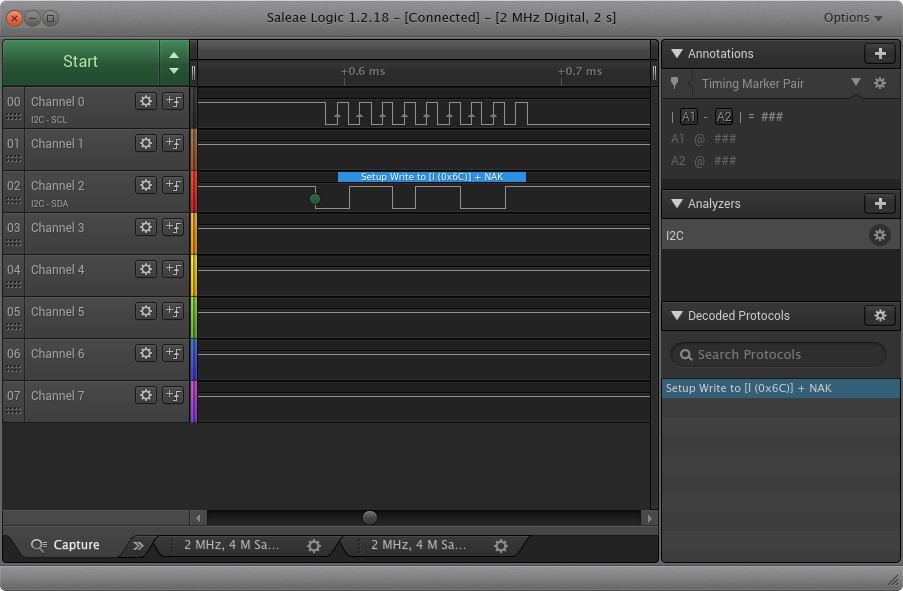
\includegraphics[width=\columnwidth]{figures/v05/waveform-i2c-1.png}
%        \caption{Waveform of the I2C port 1.}
%        \label{fig:waveform-i2c-1}
%    \end{center}
%\end{figure}

\begin{figure}[!htb]
    \begin{center}
        \subfigure[Connections of the I$^{2}$C port 2 test.\label{fig:connections-i2c-2}]{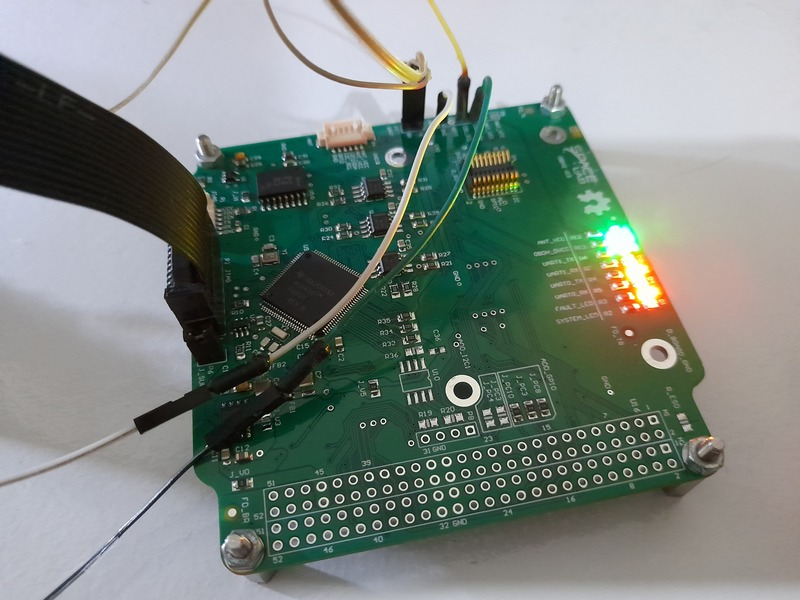
\includegraphics[height=0.22\textheight]{figures/v05/test-i2c-2.jpg}}
        ~
        \subfigure[Waveforms of the I$^{2}$C port 2 test.\label{fig:waveform-i2c-2}]{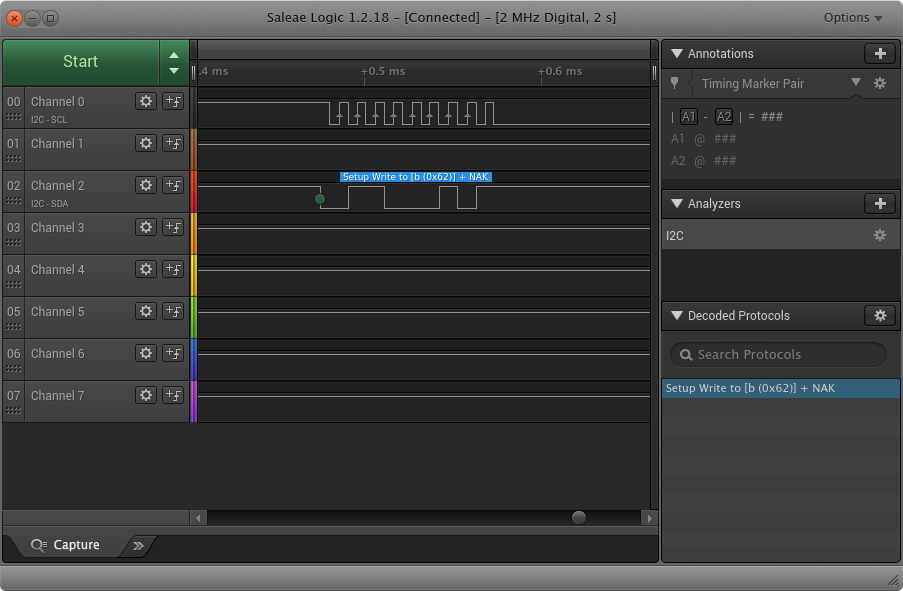
\includegraphics[height=0.22\textheight]{figures/v05/waveform-i2c-2.png}}
        \caption{I$^{2}$C port 2 test.}
        \label{fig:test-i2c-2}
    \end{center}
\end{figure}

%\begin{figure}[!ht]
%    \begin{center}
%        \includegraphics[width=0.7\columnwidth]{figures/v05/test-i2c-2.jpg}
%        \caption{Connections of the I2C port 2 test.}
%        \label{fig:test-i2c-2}
%    \end{center}
%\end{figure}
%
%\begin{figure}[!ht]
%    \begin{center}
%        \includegraphics[width=\columnwidth]{figures/v05/waveform-i2c-2.png}
%        \caption{Waveform of the I2C port 2.}
%        \label{fig:waveform-i2c-2}
%    \end{center}
%\end{figure}

\section{Sensors}

\subsection{Input Voltage}

\begin{itemize}
    \item \textbf{Test description/Objective}: .
    \item \textbf{Material}:
        \begin{itemize}
            \item Code Composer Studio v9.3.0
            \item MSP-FET Flash Emulation Tool
            \item USB-UART converter
            \item Screen (Linux software)
        \end{itemize}
    \item \textbf{Results}: .
    \item \textbf{Conclusion:} .
\end{itemize}

\subsection{Input Current}

\begin{itemize}
    \item \textbf{Test description/Objective}: .
    \item \textbf{Material}:
        \begin{itemize}
            \item Code Composer Studio v9.3.0
            \item MSP-FET Flash Emulation Tool
            \item USB-UART converter
            \item Screen (Linux software)
        \end{itemize}
    \item \textbf{Results}: .
    \item \textbf{Conclusion:} .
\end{itemize}

\begin{figure}[!htb]
    \begin{center}
        \subfigure[Current sensing circuit.\label{fig:current-sensing-circuit-v05}]{\includegraphics[width=0.8\textwidth]{figures/v05/current-sensor-circuit.png}}

        \subfigure[MAX9934 pinout.\label{fig:max9934-pinout}]{\includegraphics[width=0.4\textwidth]{figures/v05/max9934-top-view.png}}
        ~
        \subfigure[Current sensing layout (bottom layer).\label{fig:}]{\includegraphics[width=0.4\textwidth]{figures/v05/current-sensor-layout.png}}
        \caption{.}
        \label{fig:current-sensing-error-v05}
    \end{center}
\end{figure}

\begin{figure}[!ht]
    \begin{center}
        \includegraphics[width=0.6\columnwidth]{figures/v05/max9934-fix.jpg}
        \caption{Current sensor fix.}
        \label{fig:current-sensor-fix}
    \end{center}
\end{figure}

\begin{figure}[!ht]
    \begin{center}
        \includegraphics[width=0.7\columnwidth]{figures/v05/log-current-sensor.png}
        \caption{Log messages with the read values from the current sensor.}
        \label{fig:log-current-sensor}
    \end{center}
\end{figure}

\section{Peripherals}

\subsection{NOR Flash Memory}

\begin{itemize}
    \item \textbf{Test description/Objective}: Test the functionality of the NOR flash memory by verifying the device ID register of the IC.
    \item \textbf{Material}:
        \begin{itemize}
            \item Saleae Logic Analyzer (24 MHz, 8 channels)
            \item Saleae Logic software (v1.2.18)
            \item MSP-FET Flash Emulation Tool
        \end{itemize}
    \item \textbf{Results}: The results of this test can be seen in \autoref{fig:test-nor-memory}.
    \item \textbf{Conclusion:} No problems were identified on this test, as can be seen in Figure \ref{fig:waveform-spi-mem}, the device ID register was read as expected.
\end{itemize}

\begin{figure}[!htb]
    \begin{center}
        \subfigure[Connections of the NOR flash memory test.\label{fig:connections-nor-memory}]{\includegraphics[height=0.22\textheight]{figures/v05/test-nor-memory.jpg}}
        ~
        \subfigure[Waveforms of the NOR memory SPI.\label{fig:waveform-spi-mem}]{\includegraphics[height=0.22\textheight]{figures/v05/waveform-spi-mem.png}}
        \caption{NOR memory SPI test.}
        \label{fig:test-nor-memory}
    \end{center}
\end{figure}

%\begin{figure}[!ht]
%    \begin{center}
%        \includegraphics[width=0.7\columnwidth]{figures/v05/test-nor-memory.jpg}
%        \caption{Connections of the NOR flash memory test.}
%        \label{fig:test-nor-memory}
%    \end{center}
%\end{figure}
%
%\begin{figure}[!ht]
%    \begin{center}
%        \includegraphics[width=\columnwidth]{figures/v05/waveform-spi-mem.png}
%        \caption{Waveform of the NOR memory SPI.}
%        \label{fig:waveform-spi-mem}
%    \end{center}
%\end{figure}

\section{Conclusion}

Excluding the current sensor issue, no major problems were identified during the executed tests. For the next fabrication round, the identified mistakes will be corrected.


\end{appendices}


\end{document}
